%%%%%%%%%%%%%%%%%%%%%%%%%%%%%%%%%%%%%%%%%
% The Legrand Orange Book
% LaTeX Template
% Version 2.1.1 (14/2/16)
%
% This template has been downloaded from:
% http://www.LaTeXTemplates.com
%
% Original author:
% Mathias Legrand (legrand.mathias@gmail.com) with modifications by:
% Vel (vel@latextemplates.com)
%
% License:
% CC BY-NC-SA 3.0 (http://creativecommons.org/licenses/by-nc-sa/3.0/)
%
% Compiling this template:
% This template uses biber for its bibliography and makeindex for its index.
% When you first open the template, compile it from the command line with the
% commands below to make sure your LaTeX distribution is configured correctly:
%
% 1) pdflatex main
% 2) makeindex main.idx -s StyleInd.ist
% 3) biber main
% 4) pdflatex main x 2
%
% After this, when you wish to update the bibliography/index use the appropriate
% command above and make sure to compile with pdflatex several times
% afterwards to propagate your changes to the document.
%
% This template also uses a number of packages which may need to be
% updated to the newest versions for the template to compile. It is strongly
% recommended you update your LaTeX distribution if you have any
% compilation errors.
%
% Important note:
% Chapter heading images should have a 2:1 width:height ratio,
% e.g. 920px width and 460px height.
%
%%%%%%%%%%%%%%%%%%%%%%%%%%%%%%%%%%%%%%%%%

%----------------------------------------------------------------------------------------
%	PACKAGES AND OTHER DOCUMENT CONFIGURATIONS
%----------------------------------------------------------------------------------------

\documentclass[11pt,fleqn]{book} % Default font size and left-justified equations

\usepackage{listings}
\usepackage{minted}
%----------------------------------------------------------------------------------------

%%%%%%%%%%%%%%%%%%%%%%%%%%%%%%%%%%%%%%%%%
% The Legrand Orange Book
% Structural Definitions File
% Version 2.0 (9/2/15)
%
% Original author:
% Mathias Legrand (legrand.mathias@gmail.com) with modifications by:
% Vel (vel@latextemplates.com)
%
% This file has been downloaded from:
% http://www.LaTeXTemplates.com
%
% License:
% CC BY-NC-SA 3.0 (http://creativecommons.org/licenses/by-nc-sa/3.0/)
%
%%%%%%%%%%%%%%%%%%%%%%%%%%%%%%%%%%%%%%%%%

%----------------------------------------------------------------------------------------
%	VARIOUS REQUIRED PACKAGES AND CONFIGURATIONS
%----------------------------------------------------------------------------------------

\usepackage[top=3cm,bottom=3cm,left=3cm,right=3cm,headsep=10pt,a4paper]{geometry} % Page margins

\usepackage{kotex}
\usepackage{graphicx} % Required for including pictures
\graphicspath{{Pictures/}} % Specifies the directory where pictures are stored

\usepackage{lipsum} % Inserts dummy text

\usepackage{tikz} % Required for drawing custom shapes

\usepackage[english]{babel} % English language/hyphenation

\usepackage{enumitem} % Customize lists
\setlist{nolistsep} % Reduce spacing between bullet points and numbered lists

\usepackage{booktabs} % Required for nicer horizontal rules in tables

\usepackage{xcolor} % Required for specifying colors by name
\definecolor{ocre}{RGB}{243,102,25} % Define the orange color used for highlighting throughout the book

%----------------------------------------------------------------------------------------
%	FONTS
%----------------------------------------------------------------------------------------

\usepackage{avant} % Use the Avantgarde font for headings
%\usepackage{times} % Use the Times font for headings
\usepackage{mathptmx} % Use the Adobe Times Roman as the default text font together with math symbols from the Sym­bol, Chancery and Com­puter Modern fonts

\usepackage{microtype} % Slightly tweak font spacing for aesthetics
\usepackage[utf8]{inputenc} % Required for including letters with accents
\usepackage[T1]{fontenc} % Use 8-bit encoding that has 256 glyphs

%----------------------------------------------------------------------------------------
%	BIBLIOGRAPHY AND INDEX
%----------------------------------------------------------------------------------------

\usepackage[style=alphabetic,citestyle=numeric,sorting=nyt,sortcites=true,autopunct=true,babel=hyphen,hyperref=true,abbreviate=false,backref=true,backend=biber]{biblatex}
\addbibresource{bibliography.bib} % BibTeX bibliography file
\defbibheading{bibempty}{}

\usepackage{calc} % For simpler calculation - used for spacing the index letter headings correctly
\usepackage{makeidx} % Required to make an index
\makeindex % Tells LaTeX to create the files required for indexing

%----------------------------------------------------------------------------------------
%	MAIN TABLE OF CONTENTS
%----------------------------------------------------------------------------------------

\usepackage{titletoc} % Required for manipulating the table of contents

\contentsmargin{0cm} % Removes the default margin

% Part text styling
\titlecontents{part}[0cm]
{\addvspace{20pt}\centering\large\bfseries}
{}
{}
{}

% Chapter text styling
\titlecontents{chapter}[1.25cm] % Indentation
{\addvspace{12pt}\large\sffamily\bfseries} % Spacing and font options for chapters
{\color{ocre!60}\contentslabel[\Large\thecontentslabel]{1.25cm}\color{ocre}} % Chapter number
{\color{ocre}}
{\color{ocre!60}\normalsize\;\titlerule*[.5pc]{.}\;\thecontentspage} % Page number

% Section text styling
\titlecontents{section}[1.25cm] % Indentation
{\addvspace{3pt}\sffamily\bfseries} % Spacing and font options for sections
{\contentslabel[\thecontentslabel]{1.25cm}} % Section number
{}
{\hfill\color{black}\thecontentspage} % Page number
[]

% Subsection text styling
\titlecontents{subsection}[1.25cm] % Indentation
{\addvspace{1pt}\sffamily\small} % Spacing and font options for subsections
{\contentslabel[\thecontentslabel]{1.25cm}} % Subsection number
{}
{\ \titlerule*[.5pc]{.}\;\thecontentspage} % Page number
[]

% List of figures
\titlecontents{figure}[0em]
{\addvspace{-5pt}\sffamily}
{\thecontentslabel\hspace*{1em}}
{}
{\ \titlerule*[.5pc]{.}\;\thecontentspage}
[]

% List of tables
\titlecontents{table}[0em]
{\addvspace{-5pt}\sffamily}
{\thecontentslabel\hspace*{1em}}
{}
{\ \titlerule*[.5pc]{.}\;\thecontentspage}
[]

%----------------------------------------------------------------------------------------
%	MINI TABLE OF CONTENTS IN PART HEADS
%----------------------------------------------------------------------------------------

% Chapter text styling
\titlecontents{lchapter}[0em] % Indenting
{\addvspace{15pt}\large\sffamily\bfseries} % Spacing and font options for chapters
{\color{ocre}\contentslabel[\Large\thecontentslabel]{1.25cm}\color{ocre}} % Chapter number
{}
{\color{ocre}\normalsize\sffamily\bfseries\;\titlerule*[.5pc]{.}\;\thecontentspage} % Page number

% Section text styling
\titlecontents{lsection}[0em] % Indenting
{\sffamily\small} % Spacing and font options for sections
{\contentslabel[\thecontentslabel]{1.25cm}} % Section number
{}
{}

% Subsection text styling
\titlecontents{lsubsection}[.5em] % Indentation
{\normalfont\footnotesize\sffamily} % Font settings
{}
{}
{}

%----------------------------------------------------------------------------------------
%	PAGE HEADERS
%----------------------------------------------------------------------------------------

\usepackage{fancyhdr} % Required for header and footer configuration

\pagestyle{fancy}
\renewcommand{\chaptermark}[1]{\markboth{\sffamily\normalsize\bfseries\chaptername\ \thechapter.\ #1}{}} % Chapter text font settings
\renewcommand{\sectionmark}[1]{\markright{\sffamily\normalsize\thesection\hspace{5pt}#1}{}} % Section text font settings
\fancyhf{} \fancyhead[LE,RO]{\sffamily\normalsize\thepage} % Font setting for the page number in the header
\fancyhead[LO]{\rightmark} % Print the nearest section name on the left side of odd pages
\fancyhead[RE]{\leftmark} % Print the current chapter name on the right side of even pages
\renewcommand{\headrulewidth}{0.5pt} % Width of the rule under the header
\addtolength{\headheight}{2.5pt} % Increase the spacing around the header slightly
\renewcommand{\footrulewidth}{0pt} % Removes the rule in the footer
\fancypagestyle{plain}{\fancyhead{}\renewcommand{\headrulewidth}{0pt}} % Style for when a plain pagestyle is specified

% Removes the header from odd empty pages at the end of chapters
\makeatletter
\renewcommand{\cleardoublepage}{
\clearpage\ifodd\c@page\else
\hbox{}
\vspace*{\fill}
\thispagestyle{empty}
\newpage
\fi}

%----------------------------------------------------------------------------------------
%	THEOREM STYLES
%----------------------------------------------------------------------------------------

\usepackage{amsmath,amsfonts,amssymb,amsthm} % For math equations, theorems, symbols, etc

\newcommand{\intoo}[2]{\mathopen{]}#1\,;#2\mathclose{[}}
\newcommand{\ud}{\mathop{\mathrm{{}d}}\mathopen{}}
\newcommand{\intff}[2]{\mathopen{[}#1\,;#2\mathclose{]}}
\newtheorem{notation}{Notation}[chapter]

% Boxed/framed environments
\newtheoremstyle{ocrenumbox}% % Theorem style name
{0pt}% Space above
{0pt}% Space below
{\normalfont}% % Body font
{}% Indent amount
{\small\bf\sffamily\color{ocre}}% % Theorem head font
{\;}% Punctuation after theorem head
{0.25em}% Space after theorem head
{\small\sffamily\color{ocre}\thmname{#1}\nobreakspace\thmnumber{\@ifnotempty{#1}{}\@upn{#2}}% Theorem text (e.g. Theorem 2.1)
\thmnote{\nobreakspace\the\thm@notefont\sffamily\bfseries\color{black}---\nobreakspace#3.}} % Optional theorem note
\renewcommand{\qedsymbol}{$\blacksquare$}% Optional qed square

\newtheoremstyle{blacknumex}% Theorem style name
{5pt}% Space above
{5pt}% Space below
{\normalfont}% Body font
{} % Indent amount
{\small\bf\sffamily}% Theorem head font
{\;}% Punctuation after theorem head
{0.25em}% Space after theorem head
{\small\sffamily{\tiny\ensuremath{\blacksquare}}\nobreakspace\thmname{#1}\nobreakspace\thmnumber{\@ifnotempty{#1}{}\@upn{#2}}% Theorem text (e.g. Theorem 2.1)
\thmnote{\nobreakspace\the\thm@notefont\sffamily\bfseries---\nobreakspace#3.}}% Optional theorem note

\newtheoremstyle{blacknumbox} % Theorem style name
{0pt}% Space above
{0pt}% Space below
{\normalfont}% Body font
{}% Indent amount
{\small\bf\sffamily}% Theorem head font
{\;}% Punctuation after theorem head
{0.25em}% Space after theorem head
{\small\sffamily\thmname{#1}\nobreakspace\thmnumber{\@ifnotempty{#1}{}\@upn{#2}}% Theorem text (e.g. Theorem 2.1)
\thmnote{\nobreakspace\the\thm@notefont\sffamily\bfseries---\nobreakspace#3.}}% Optional theorem note

% Non-boxed/non-framed environments
\newtheoremstyle{ocrenum}% % Theorem style name
{5pt}% Space above
{5pt}% Space below
{\normalfont}% % Body font
{}% Indent amount
{\small\bf\sffamily\color{ocre}}% % Theorem head font
{\;}% Punctuation after theorem head
{0.25em}% Space after theorem head
{\small\sffamily\color{ocre}\thmname{#1}\nobreakspace\thmnumber{\@ifnotempty{#1}{}\@upn{#2}}% Theorem text (e.g. Theorem 2.1)
\thmnote{\nobreakspace\the\thm@notefont\sffamily\bfseries\color{black}---\nobreakspace#3.}} % Optional theorem note
\renewcommand{\qedsymbol}{$\blacksquare$}% Optional qed square
\makeatother

% Defines the theorem text style for each type of theorem to one of the three styles above
\newcounter{dummy}
\numberwithin{dummy}{section}
\theoremstyle{ocrenumbox}
\newtheorem{theoremeT}[dummy]{Theorem}
\newtheorem{problem}{Problem}[chapter]
\newtheorem{exerciseT}{Exercise}[chapter]
\theoremstyle{blacknumex}
\newtheorem{exampleT}{Example}[chapter]
\theoremstyle{blacknumbox}
\newtheorem{vocabulary}{Vocabulary}[chapter]
\newtheorem{definitionT}{Definition}[section]
\newtheorem{corollaryT}[dummy]{Corollary}
\theoremstyle{ocrenum}
\newtheorem{proposition}[dummy]{Proposition}

%----------------------------------------------------------------------------------------
%	DEFINITION OF COLORED BOXES
%----------------------------------------------------------------------------------------

\RequirePackage[framemethod=default]{mdframed} % Required for creating the theorem, definition, exercise and corollary boxes

% Theorem box
\newmdenv[skipabove=7pt,
skipbelow=7pt,
backgroundcolor=black!5,
linecolor=ocre,
innerleftmargin=5pt,
innerrightmargin=5pt,
innertopmargin=5pt,
leftmargin=0cm,
rightmargin=0cm,
innerbottommargin=5pt]{tBox}

% Exercise box
\newmdenv[skipabove=7pt,
skipbelow=7pt,
rightline=false,
leftline=true,
topline=false,
bottomline=false,
backgroundcolor=ocre!10,
linecolor=ocre,
innerleftmargin=5pt,
innerrightmargin=5pt,
innertopmargin=5pt,
innerbottommargin=5pt,
leftmargin=0cm,
rightmargin=0cm,
linewidth=4pt]{eBox}

% Definition box
\newmdenv[skipabove=7pt,
skipbelow=7pt,
rightline=false,
leftline=true,
topline=false,
bottomline=false,
linecolor=ocre,
innerleftmargin=5pt,
innerrightmargin=5pt,
innertopmargin=0pt,
leftmargin=0cm,
rightmargin=0cm,
linewidth=4pt,
innerbottommargin=0pt]{dBox}

% Corollary box
\newmdenv[skipabove=7pt,
skipbelow=7pt,
rightline=false,
leftline=true,
topline=false,
bottomline=false,
linecolor=gray,
backgroundcolor=black!5,
innerleftmargin=5pt,
innerrightmargin=5pt,
innertopmargin=5pt,
leftmargin=0cm,
rightmargin=0cm,
linewidth=4pt,
innerbottommargin=5pt]{cBox}

% Creates an environment for each type of theorem and assigns it a theorem text style from the "Theorem Styles" section above and a colored box from above
\newenvironment{theorem}{\begin{tBox}\begin{theoremeT}}{\end{theoremeT}\end{tBox}}
\newenvironment{exercise}{\begin{eBox}\begin{exerciseT}}{\hfill{\color{ocre}\tiny\ensuremath{\blacksquare}}\end{exerciseT}\end{eBox}}
\newenvironment{definition}{\begin{dBox}\begin{definitionT}}{\end{definitionT}\end{dBox}}
\newenvironment{example}{\begin{exampleT}}{\hfill{\tiny\ensuremath{\blacksquare}}\end{exampleT}}
\newenvironment{corollary}{\begin{cBox}\begin{corollaryT}}{\end{corollaryT}\end{cBox}}

%----------------------------------------------------------------------------------------
%	REMARK ENVIRONMENT
%----------------------------------------------------------------------------------------

\newenvironment{remark}{\par\vspace{10pt}\small % Vertical white space above the remark and smaller font size
\begin{list}{}{
\leftmargin=35pt % Indentation on the left
\rightmargin=25pt}\item\ignorespaces % Indentation on the right
\makebox[-2.5pt]{\begin{tikzpicture}[overlay]
\node[draw=ocre!60,line width=1pt,circle,fill=ocre!25,font=\sffamily\bfseries,inner sep=2pt,outer sep=0pt] at (-15pt,0pt){\textcolor{ocre}{R}};\end{tikzpicture}} % Orange R in a circle
\advance\baselineskip -1pt}{\end{list}\vskip5pt} % Tighter line spacing and white space after remark

%----------------------------------------------------------------------------------------
%	SECTION NUMBERING IN THE MARGIN
%----------------------------------------------------------------------------------------

\makeatletter
\renewcommand{\@seccntformat}[1]{\llap{\textcolor{ocre}{\csname the#1\endcsname}\hspace{1em}}}
\renewcommand{\section}{\@startsection{section}{1}{\z@}
{-4ex \@plus -1ex \@minus -.4ex}
{1ex \@plus.2ex }
{\normalfont\large\sffamily\bfseries}}
\renewcommand{\subsection}{\@startsection {subsection}{2}{\z@}
{-3ex \@plus -0.1ex \@minus -.4ex}
{0.5ex \@plus.2ex }
{\normalfont\sffamily\bfseries}}
\renewcommand{\subsubsection}{\@startsection {subsubsection}{3}{\z@}
{-2ex \@plus -0.1ex \@minus -.2ex}
{.2ex \@plus.2ex }
{\normalfont\small\sffamily\bfseries}}
\renewcommand\paragraph{\@startsection{paragraph}{4}{\z@}
{-2ex \@plus-.2ex \@minus .2ex}
{.1ex}
{\normalfont\small\sffamily\bfseries}}

%----------------------------------------------------------------------------------------
%	PART HEADINGS
%----------------------------------------------------------------------------------------

% numbered part in the table of contents
\newcommand{\@mypartnumtocformat}[2]{%
\setlength\fboxsep{0pt}%
\noindent\colorbox{ocre!20}{\strut\parbox[c][.7cm]{\ecart}{\color{ocre!70}\Large\sffamily\bfseries\centering#1}}\hskip\esp\colorbox{ocre!40}{\strut\parbox[c][.7cm]{\linewidth-\ecart-\esp}{\Large\sffamily\centering#2}}}%
%%%%%%%%%%%%%%%%%%%%%%%%%%%%%%%%%%
% unnumbered part in the table of contents
\newcommand{\@myparttocformat}[1]{%
\setlength\fboxsep{0pt}%
\noindent\colorbox{ocre!40}{\strut\parbox[c][.7cm]{\linewidth}{\Large\sffamily\centering#1}}}%
%%%%%%%%%%%%%%%%%%%%%%%%%%%%%%%%%%
\newlength\esp
\setlength\esp{4pt}
\newlength\ecart
\setlength\ecart{1.2cm-\esp}
\newcommand{\thepartimage}{}%
\newcommand{\partimage}[1]{\renewcommand{\thepartimage}{#1}}%
\def\@part[#1]#2{%
\ifnum \c@secnumdepth >-2\relax%
\refstepcounter{part}%
\addcontentsline{toc}{part}{\texorpdfstring{\protect\@mypartnumtocformat{\thepart}{#1}}{\partname~\thepart\ ---\ #1}}
\else%
\addcontentsline{toc}{part}{\texorpdfstring{\protect\@myparttocformat{#1}}{#1}}%
\fi%
\startcontents%
\markboth{}{}%
{\thispagestyle{empty}%
\begin{tikzpicture}[remember picture,overlay]%
\node at (current page.north west){\begin{tikzpicture}[remember picture,overlay]%
\fill[ocre!20](0cm,0cm) rectangle (\paperwidth,-\paperheight);
\node[anchor=north] at (4cm,-3.25cm){\color{ocre!40}\fontsize{220}{100}\sffamily\bfseries\@Roman\c@part};
\node[anchor=south east] at (\paperwidth-1cm,-\paperheight+1cm){\parbox[t][][t]{8.5cm}{
\printcontents{l}{0}{\setcounter{tocdepth}{1}}%
}};
\node[anchor=north east] at (\paperwidth-1.5cm,-3.25cm){\parbox[t][][t]{15cm}{\strut\raggedleft\color{white}\fontsize{30}{30}\sffamily\bfseries#2}};
\end{tikzpicture}};
\end{tikzpicture}}%
\@endpart}
\def\@spart#1{%
\startcontents%
\phantomsection
{\thispagestyle{empty}%
\begin{tikzpicture}[remember picture,overlay]%
\node at (current page.north west){\begin{tikzpicture}[remember picture,overlay]%
\fill[ocre!20](0cm,0cm) rectangle (\paperwidth,-\paperheight);
\node[anchor=north east] at (\paperwidth-1.5cm,-3.25cm){\parbox[t][][t]{15cm}{\strut\raggedleft\color{white}\fontsize{30}{30}\sffamily\bfseries#1}};
\end{tikzpicture}};
\end{tikzpicture}}
\addcontentsline{toc}{part}{\texorpdfstring{%
\setlength\fboxsep{0pt}%
\noindent\protect\colorbox{ocre!40}{\strut\protect\parbox[c][.7cm]{\linewidth}{\Large\sffamily\protect\centering #1\quad\mbox{}}}}{#1}}%
\@endpart}
\def\@endpart{\vfil\newpage
\if@twoside
\if@openright
\null
\thispagestyle{empty}%
\newpage
\fi
\fi
\if@tempswa
\twocolumn
\fi}

%----------------------------------------------------------------------------------------
%	CHAPTER HEADINGS
%----------------------------------------------------------------------------------------

% A switch to conditionally include a picture, implemented by  Christian Hupfer
\newif\ifusechapterimage
\usechapterimagetrue
\newcommand{\thechapterimage}{}%
\newcommand{\chapterimage}[1]{\ifusechapterimage\renewcommand{\thechapterimage}{#1}\fi}%
\def\@makechapterhead#1{%
{\parindent \z@ \raggedright \normalfont
\ifnum \c@secnumdepth >\m@ne
\if@mainmatter
\begin{tikzpicture}[remember picture,overlay]
\node at (current page.north west)
{\begin{tikzpicture}[remember picture,overlay]
\node[anchor=north west,inner sep=0pt] at (0,0) {\ifusechapterimage\includegraphics[width=\paperwidth]{\thechapterimage}\fi};
\draw[anchor=west] (\Gm@lmargin,-9cm) node [line width=2pt,rounded corners=15pt,draw=ocre,fill=white,fill opacity=0.5,inner sep=15pt]{\strut\makebox[22cm]{}};
\draw[anchor=west] (\Gm@lmargin+.3cm,-9cm) node {\huge\sffamily\bfseries\color{black}\thechapter. #1\strut};
\end{tikzpicture}};
\end{tikzpicture}
\else
\begin{tikzpicture}[remember picture,overlay]
\node at (current page.north west)
{\begin{tikzpicture}[remember picture,overlay]
\node[anchor=north west,inner sep=0pt] at (0,0) {\ifusechapterimage\includegraphics[width=\paperwidth]{\thechapterimage}\fi};
\draw[anchor=west] (\Gm@lmargin,-9cm) node [line width=2pt,rounded corners=15pt,draw=ocre,fill=white,fill opacity=0.5,inner sep=15pt]{\strut\makebox[22cm]{}};
\draw[anchor=west] (\Gm@lmargin+.3cm,-9cm) node {\huge\sffamily\bfseries\color{black}#1\strut};
\end{tikzpicture}};
\end{tikzpicture}
\fi\fi\par\vspace*{270\p@}}}

%-------------------------------------------

\def\@makeschapterhead#1{%
\begin{tikzpicture}[remember picture,overlay]
\node at (current page.north west)
{\begin{tikzpicture}[remember picture,overlay]
\node[anchor=north west,inner sep=0pt] at (0,0) {\ifusechapterimage\includegraphics[width=\paperwidth]{\thechapterimage}\fi};
\draw[anchor=west] (\Gm@lmargin,-9cm) node [line width=2pt,rounded corners=15pt,draw=ocre,fill=white,fill opacity=0.5,inner sep=15pt]{\strut\makebox[22cm]{}};
\draw[anchor=west] (\Gm@lmargin+.3cm,-9cm) node {\huge\sffamily\bfseries\color{black}#1\strut};
\end{tikzpicture}};
\end{tikzpicture}
\par\vspace*{270\p@}}
\makeatother

%----------------------------------------------------------------------------------------
%	HYPERLINKS IN THE DOCUMENTS
%----------------------------------------------------------------------------------------

\usepackage{hyperref}
\hypersetup{hidelinks,backref=true,pagebackref=true,hyperindex=true,colorlinks=false,breaklinks=true,urlcolor= ocre,bookmarks=true,bookmarksopen=false,pdftitle={Title},pdfauthor={Author}}
\usepackage{bookmark}
\bookmarksetup{
open,
numbered,
addtohook={%
\ifnum\bookmarkget{level}=0 % chapter
\bookmarksetup{bold}%
\fi
\ifnum\bookmarkget{level}=-1 % part
\bookmarksetup{color=ocre,bold}%
\fi
}
}
 % Insert the commands.tex file which contains the majority of the structure behind the template

\begin{document}

%----------------------------------------------------------------------------------------
%	TITLE PAGE
%----------------------------------------------------------------------------------------

\begingroup
\thispagestyle{empty}
\begin{tikzpicture}[remember picture,overlay]
\coordinate [below=12cm] (midpoint) at (current page.north);
\node at (current page.north west)
{\begin{tikzpicture}[remember picture,overlay]
\node[anchor=north west,inner sep=0pt] at (0,0) {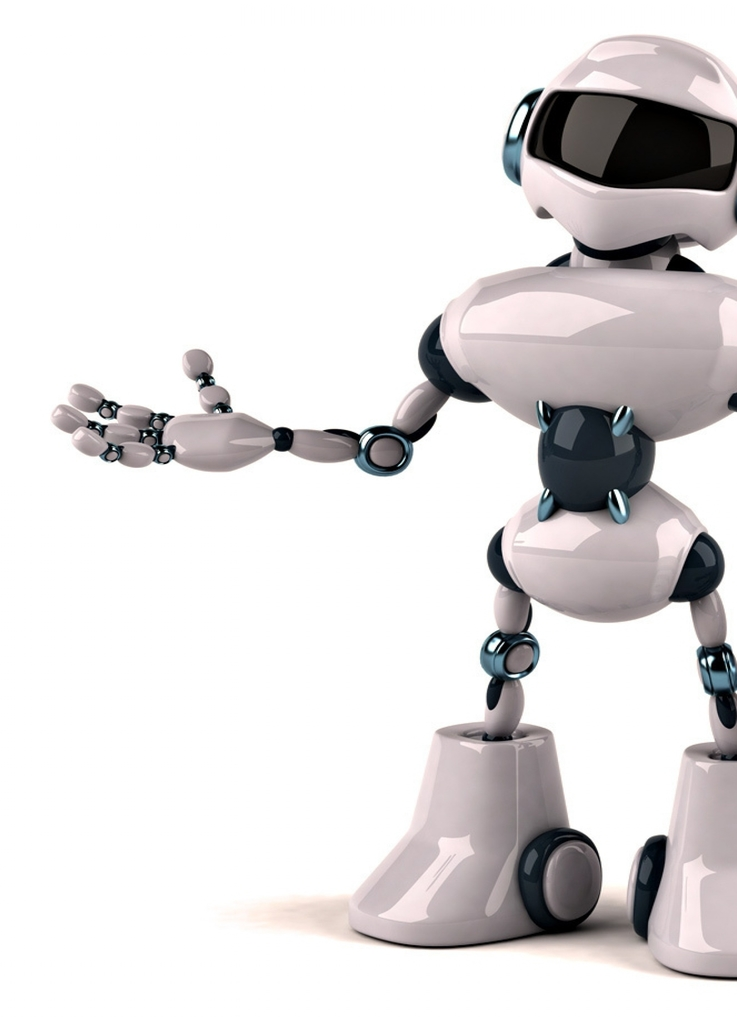
\includegraphics[width=\paperwidth]{robotics-wp}}; % Background image
\draw[anchor=north] (midpoint) node [fill=ocre!30!white,fill opacity=0.6,text opacity=1,inner sep=1cm]{\Huge\centering\bfseries\sffamily\parbox[c][][t]{\paperwidth}{\centering 실전 ROS 시스템 구축\\[30pt] % Book title
{\Large Python, Matlab을 이용한 ROS}\\[20pt] % Subtitle
{\huge Donghoon Park}}}; % Author name
\end{tikzpicture}};
\end{tikzpicture}
\vfill
\endgroup

%----------------------------------------------------------------------------------------
%	COPYRIGHT PAGE
%----------------------------------------------------------------------------------------

\newpage
~\vfill
\thispagestyle{empty}

\noindent Copyright \copyright\ 2016 Donghoon Park\\ % Copyright notice

\noindent \textsc{Published by Publisher}\\ % Publisher

\noindent \textsc{sigma.snu.ac.kr}\\ % URL

\noindent GPL License

\noindent \textit{First printing, June 2016} % Printing/edition date

%----------------------------------------------------------------------------------------
%	TABLE OF CONTENTS
%----------------------------------------------------------------------------------------

%\usechapterimagefalse % If you don't want to include a chapter image, use this to toggle images off - it can be enabled later with \usechapterimagetrue

\chapterimage{chapter_head_1.pdf} % Table of contents heading image

\pagestyle{empty} % No headers

\tableofcontents % Print the table of contents itself

\cleardoublepage % Forces the first chapter to start on an odd page so it's on the right

\pagestyle{fancy} % Print headers again

%----------------------------------------------------------------------------------------
%	PART
%----------------------------------------------------------------------------------------

\part{Part1}

%----------------------------------------------------------------------------------------
%	CHAPTER 1
%----------------------------------------------------------------------------------------

\chapterimage{ros-names.png} % Chapter heading image

\chapter{ROS 개요 및 환경설정}

\section{ROS란 무엇인가}\index{Paragraphs of Text}


ROS는 Robot Operating System 으로, 로봇과 관련된 여러 패키지를 제공하고,
특히 프로시저간의 안전한 통신 규약을 제공하는 프로그램입니다.
Operating System이라는 이름 때문에 오히려 ROS의 개념에 대해 헷갈려하는 분들이 계신데,
ROS는 OS가 하는 일을 일부 도맡아서 하는 프로그램으로 생각하시면 됩니다.

ROS는 2016년 6월 시점으로 ROS Kinetic 버전까지 나와있으며, ROS의 마스코트는 왜인지 모르겠지만 거북이이고,
레퍼런스 로봇은 꼬부기(turtlebot)이고, 예제도 거북이로 시작합니다. ROS는 설치하는 과정 자체가 기존 Linux유저 기준으로 어려운 편은 아니지만,
로봇을 만드는 사람들이 모두 Linux에 익숙한 것은 아니기 때문에 설치 난이도가 낮은 편은 아닙니다.
어떻게 보면 매우 어려운 설치 과정을 거치는데, 이런 고생을 하면서까지 왜 ROS를 사용해야 하는지에 대해 이야기해보도록 하죠.


\includegraphics[scale=0.3]{ros-kinetic}

ROS의 필요성에 대해 이야기하려면 ROS가 어떤 것인지부터 이야기해야 할 것입니다.
프로그래머의 입장에서 보면, ROS는 일종의 라이브러리입니다. Python, C++, Matlab, Javascript 등에서 돌아가는 라이브러리를 공식적/ 비공식적으로 제공하며,
프로그램 언어에서 쉽게 불러와서 사용할 수 있습니다. ROS 라이브러리가 제공하는 API는 상당히 단순합니다.
데이터를 저장하고 불러오는 두 가지 방식에 대한 함수(or Functional Block)를 제공할 뿐입니다.
여기서 의문이 들 수 있습니다.리눅스에 조금 익숙하신 분이라면 알겠지만 리눅스에서는 변수 공유를 그다지 어려운 과정을 거치지 않고 할 수 있습니다.
왜 굳이 ROS를 써야 하는것일까요? 그 해답은 ROS의 호환성에 있다고 할 수 있습니다. ROS는 다른 언어간에도 심지어 다른 하드웨어간에도 변수 공유를 위한 프로토콜을 제공합니다.
그리고 무엇보다도 프로그램을 패키지화 시키고 나면, 우리가 프로그램의 내부를 아얘 모르고도 그 패키지에서 뽑아주는 변수만 사용할 수 있다는 점이 가장 큰 장점이죠.
사실상의 하드웨어 플러그 앤 플레이를 진정하게 가능하게 하는 것이죠.
ROS 패키지를 이용할 때는 소프트웨어 패키지는 설치 후 실행만 하면 됩니다. 하드웨어 연결이 필요한 패키지는 동일한 하드웨어 구성 후 꽂고, 패키지를 실행하면 됩니다.
기존에 개발한 하드웨어에 대한 완벽한 재사용성을 확보할 수 있는 것이죠.
임베디드 환경에서 구르던 로봇 프로그래머들에게 조금 더 감을 잡을 수 있게 예시를 들어보자면,
다른 사람이 짠 아두이노 시스템을 컴퓨터에 꽂기만 하면 주요 변수를 ROS가 directory 형식으로 정리해서 보여준다는 말도 안되는 일이 가능해집니다.

결론적으로, 하드웨어 및 소프트웨어의 모듈화 및 재사용성을 극한까지 추구할 수 있는 구조가 ROS라고 보시면 됩니다.


%------------------------------------------------

\section{ROS를 사용하기 위해서는?}\index{ROS를 사용하기 위해서는?}

ROS를 사용하기 위해서는 먼저 시스템을 구성해야 합니다. ROS는 보통 Ubuntu라는 리눅스 배포판 위에
올려서 쓰는 것이 일반적입니다. Ubuntu 위에서는 ROS를 비교적 쉽게 명령줄 도구를 이용해서 설치할 수 있습니다.
또한, Ubuntu는 리눅스 배포판 중 매우 유명한 축에 속하며 ARM 보드를 상당히 잘 지원하기 때문에 소형 로봇 시스템에도 올릴 수 있다는 점에서 Ubutu 위에서 ROS 구성 후 실습을 하시는 것을 권장합니다.

그리고, ROS에 접속하는 프로그램을 짜는 과정 또한 필요하기 때문에 개발용 프로그램 언어 환경 또한 설치해야 합니다.
보통 ROS 접속 프로그램을 짤 떄는 Python, C++ 등의 언어를 사용합니다. 이 책에서는 Python을 주 개발 언어로 사용하는 과정에 대해 이야기하겠습니다.
보다 나은 성능을 원한다면 C++을 이용하는 것을 권장합니다. ros 기본 메뉴얼은 C++로 작성되어있기 때문에, 기본 ros 매뉴얼을 따라서 한다면 C++ 프로그래밍은 어렵지 않게 할 수 있습니다.
이 교재에서 Python을 주 언어로 사용하는 이유는 스크립트 인터프리터를 이용한 실시간 코드 확인이 가능하기 때문입니다. 다시 한번 강조하지만 프로그램이 무거운 경우 C++에서의 개발을 권장합니다.

또한 이것은 필자의 개인적인 추천인데, Matlab을 활용할 수 있는 환경에 있고, 로봇의 Computing Power가 충분히 좋은 경우 Matlab의 Simulink를 사용하는 것을 추천합니다.
Matlab Simulink는 Gui Block Programming Language로 시스템 구성에 있어서는 매우 탁월한 기능을 갖추고 있습니다.
특히, DSP Filter 구성에서는 따라올 대안이 없다는 것에는 대부분의 엔지니어가 동의할 것입니다.

따라서 본 교재를 전부 보기 위해서는 아래와 같은 환경을 구성하고 가는 것을 추천합니다.

\begin{enumerate}
\item Ubuntu 14.04 or Ubuntu 16.04
\item ROS Jade or Kinetic
\item Python 2.7 and Development Environment
\item Matlab 2016a with Simulink Robotics Communication Block
\item Arduino or Mbed
\end{enumerate}

이제 Arduino를 제외한 (아두이노는 인간적으로 너무 쉬워요..) 해당 환경들을 설치하는 방법에 대해서 차근차근 설명해 보겠습니다.

%------------------------------------------------

%------------------------------------------------
\section{Ubuntu 설치}
\label{sec:Ubuntu 설치}

이번 섹션에서는 Ubuntu를 설치하는 방법에 대해 이야기해 보겠습니다. Ubuntu는 앞서 말했듯이 리눅스 시스템으로,
ROS를 올리기 좋은 환경을 제공해줍니다. 하드웨어를 연계해서 개발을 할 예정이니 Virtual Machine이 아닌 Native로 설치하는 것을 권장합니다.
ARM 보드 위에 설치한 Ubuntu를 가지고 교재를 진행하는 것은 권장하지 않습니다. 왜냐하면 ARM에는 지원되지 않는 ROS 패키지가 많으며, 이 교재는 64비트 x86 CPU (일반적인 Intel, AMD CPU) 기준으로 쓰여졌기 때문입니다.

먼저 Ubuntu ISO Image를 다운로드 받습니다. 우분투 공식 배포판을 활용하는 것을 추천합니다.

\begin{link}[http://www.ubuntu.com/]
  : Ubuntu 공식 홈페이지
\end{link}

 Ubuntu 공식 홈페이지에 접속하셔서 Desktop 버전을 다운로드 받으세요. LTS(Long Term Support) 버전을 사용하는 것을 추천합니다.


\begin{figure}[h]
\centering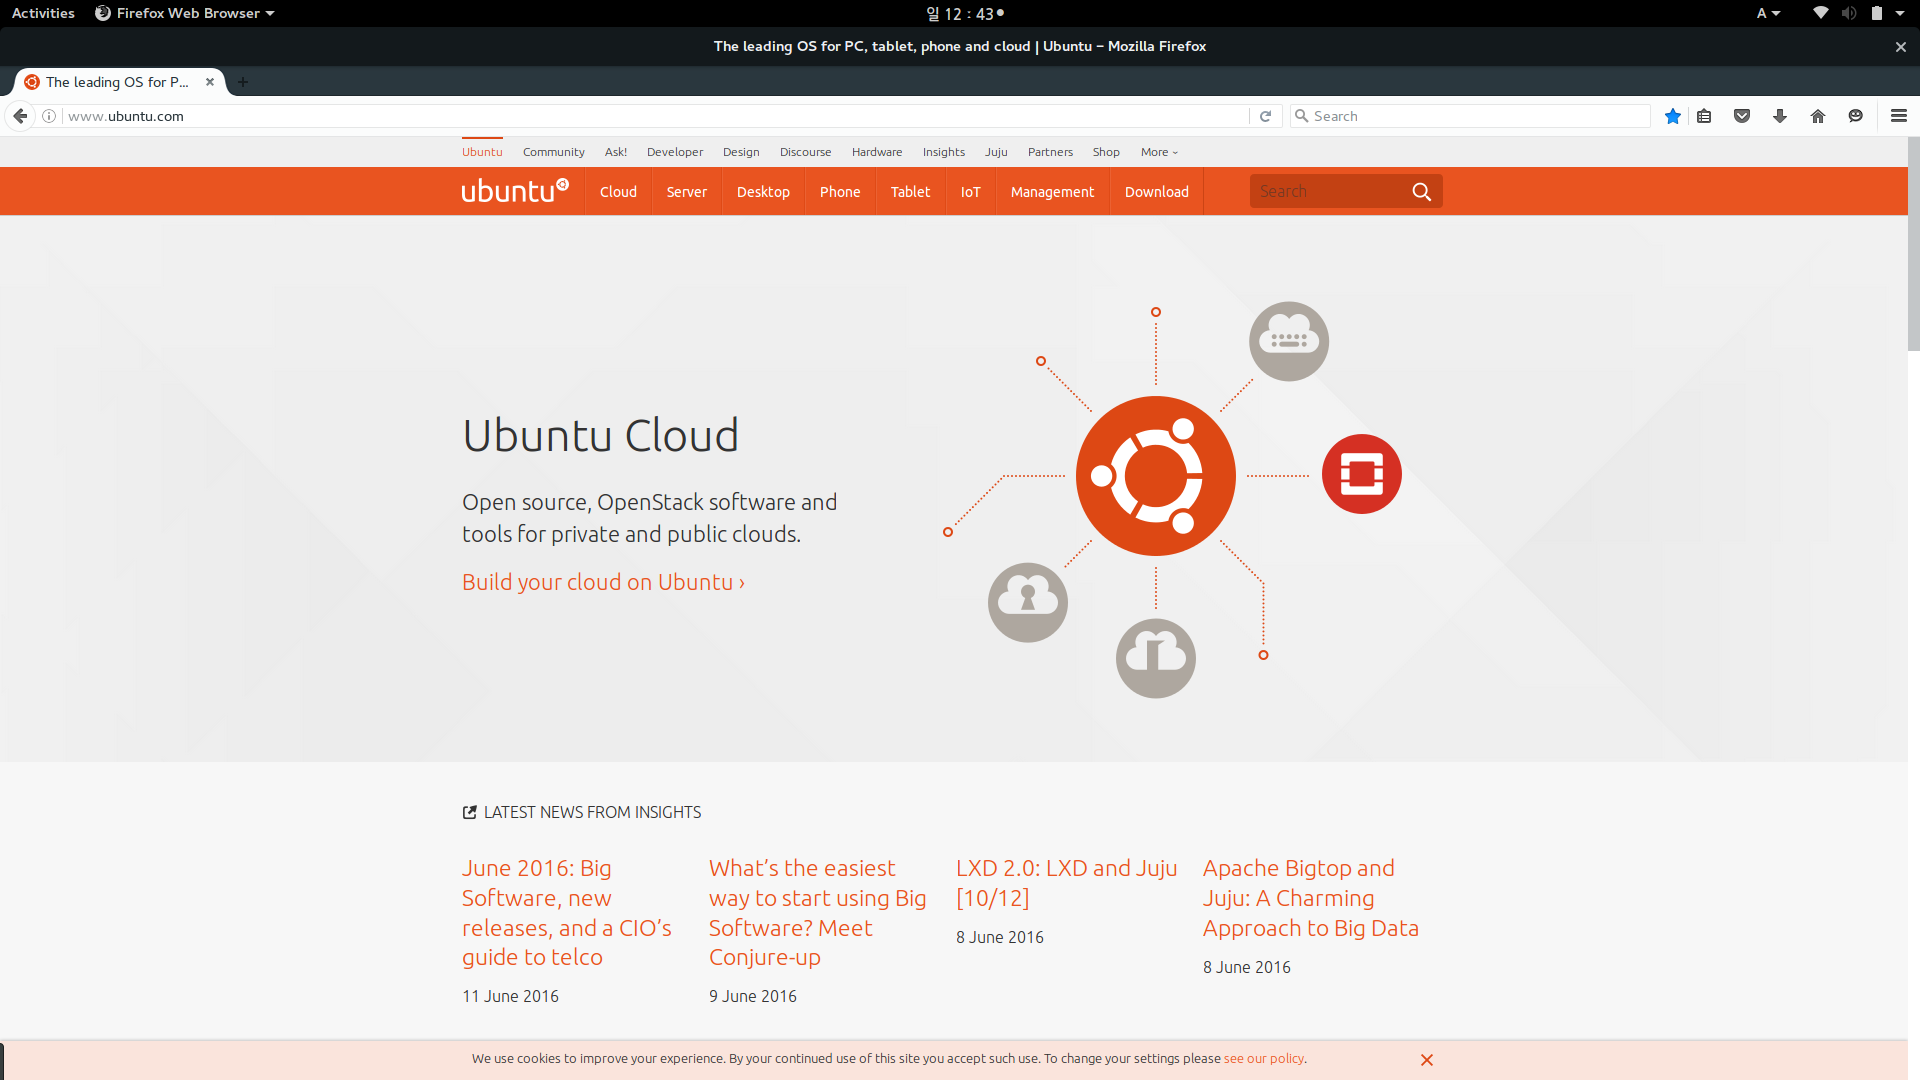
\includegraphics[scale=0.22]{01_ubuntu_mainpage}
\caption{Ubuntu 공식 페이지}
\end{figure}

다운로드 받은 ISO 파일은 이제 usb에 넣어 부팅 usb를 만들고 설치해야 합니다.
해당 과정은 잘 정리되어 있는 블로그 링크가 있기에 아래에 첨부합니다.

\begin{link}[http://sergeswin.com/1178]
: Ubuntu 부팅 usb 제작과정
\end{link}

해당 블로그의 글을 보고 부팅 usb를 만드셨다면, 이제 컴퓨터 파티션에 공간을 30GB정도 남긴 뒤(단순히 free space가 아니라 disk 관리로 들어가셔서 가용 공간을 확보하셔야 합니다.) usb로 부팅해서 해당 공간에 ubuntu를 설치하세요.
공식 홈페이지에서 튜토리얼을 제공하니 참고하셔서 설치하면 어렵지 않게 설치가 가능합니다.

\begin{link}[http://www.ubuntu.com/download/desktop/install-ubuntu-desktop]
: Ubuntu 설치 과정
\end{link}

사실 Ubuntu는 리눅스 중에서도 매우 사용자 친화적인 배포판이기 때문에 설치순서 자체가 어렵다기보다는, 설치 과정 중에 생기는 문제가 해결하기 까다롭습니다.
그러나 개인별 증상이 매우 다르고, 그 때마다 해결책도 다르기 때문에 모든 것을 매뉴얼로 만들기는 사실상 불가능합니다.
Ubuntu 설치 중에 문제가 생긴다면 아래 사이트를 참고해서 해결하도록 노력해보세요.
Linux 환경에서 작업읋 하기 위해서는 해당 배포판의 포럼을 계속해서 들락 날락 하는 노력이 필요하답니다.

\begin{link}[http://askubuntu.com/]
: AskUbuntu Forum
\end{link}

무사히 Ubuntu를 설치하셨다면 축하합니다! 다음 파트에서는 드디어 ROS를 설치해 보겠습니다.

%------------------------------------------------

\section{ROS 설치}\index{ROS 설치}

ROS는 2016.06 현재 ROS Kinetic Version 까지 나와 있습니다. ROS 또한 Ubuntu와 마찬가지로 여러 가지 배포판이 나와있는데, 일반적으로 비슷한 시기에 나온 Ubuntu와 ROS 배포판이 호환성이 좋습니다.
Ubuntu 14.04를 설치해 온 분은 ROS Jade, Ubuntu 16.04를 설치해 온 분은 ROS Kinetic을 권장합니다. 혹시나 개발기간이 촉박해서 기존 패키지를 조합하는 방식의 개발을 원하는 분은 구버전인 ROS Indigo를 사용하셔도 좋습니다.
ROS는 최신버전으로 올수록 apt-get을 이용해 간단히 설치할 수 있는 패키지가 줄어들기 때문에, 최신버전과 패키지의 숫자 사이에서 잘 저울질 해서 알맞은 버전을 선택하시길 바랍니다.

\begin{figure}[h]

\includegraphics[scale=2.0]{02_ros_indigo}

\includegraphics[scale=0.3]{03_ros_jade}

\includegraphics[scale=0.2]{04_ros_kinetic}
\caption{ROS Versions}
\end{figure}

ROS 설치를 위해서는 Ubuntu에서 커멘드 라인을 실행해야 합니다.
일반적인 환경을 구축했다면 Ctrl + Alt + T 를 누르면 아래와 같이 커멘드라인이 실행됩니다.

\begin{figure}[h]
\centering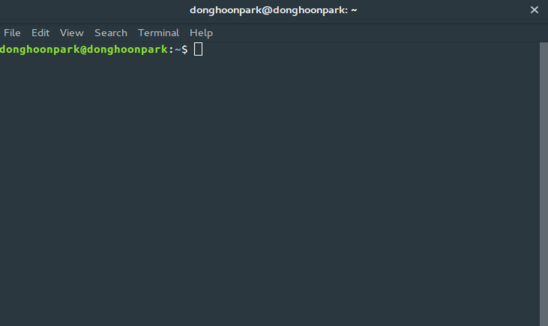
\includegraphics[scale=0.7]{05_terminal}
\caption{Terminal 실행 창}
\end{figure}

이제 이 창 위에 설치 명령어를 입력하여 ROS를 설치하게 됩니다. ROS설치는 대부분 비슷한 과정으로 진행되지만, 버전별로 약간씩 상이하기 때문에
자신이 설치할 버전이 무엇인지 잘 알고 진행하시기 바랍니다. 혹시나 ARM Linux Board(Odroid/ Raspberry pi/ Beaglebone Black)가
최종 Target System인 경우, 최신버전인 ROS Kinetic을 설치하지 않는 것을 권장합니다.

ROS의 버전별 설치 방법은 아래와 같습니다.

\begin{link}[http://wiki.ros.org/indigo/Installation/Ubuntu]
  : ROS Indigo 설치과정
\end{link}

\begin{link}[http://wiki.ros.org/jade/Installation/Ubuntu]
  : ROS Jade 설치과정
\end{link}

\begin{link}[http://wiki.ros.org/kinetic/Installation/Ubuntu]
  : ROS Kinetic 설치과정
\end{link}

설치 과정에 따라 명령어를 입력하면 ROS가 설치됩니다. desktop-full package로 설치하는 것을 권장드리며,
최대 약 1시간까지도 걸리는 작업이므로 느긋하게 기다려 주세요.
1.1 - 1.8 까지 모든 명령어를 순서대로 입력하셔야 합니다.

간단하게 설치하고 싶으시다 혹은 리눅스 초보라 아무것도 모르겠다 하시는 분은 아래 명령어를 입력해서 ROS Indigo를 간단하게 설치하는 방법도 있습니다만 권장하지 않습니다.
해당 링크는 오픈소스 로보틱스 카페 표윤석 연구원님꼐서 만든 저장소와 스크립트입니다.

\begin{link}[http://cafe.naver.com/openrt/13991]
  : wget https://raw.githubusercontent.com/oroca/oroca-ros-pkg/master/ros\_install.sh\, \&\& chmod 755\, ./ros\_install.sh\, \&\& ./ros\_install.sh\, catkin\_ws indigo
\end{link}

ROS를 모두 설치했다면 제대로 설치되었는지 roscore 프로그램을 실행시켜 봅시다.
터미널을 열고, roscore 명령어를 아래와 같이 입력하고 실행해 보세요. 정상적으로 작동한다면 ROS 설치에 성공한 것입니다. 아래 예시는 ROS Kinetic을 설치한 예시입니다.

\begin{figure}[h]
\centering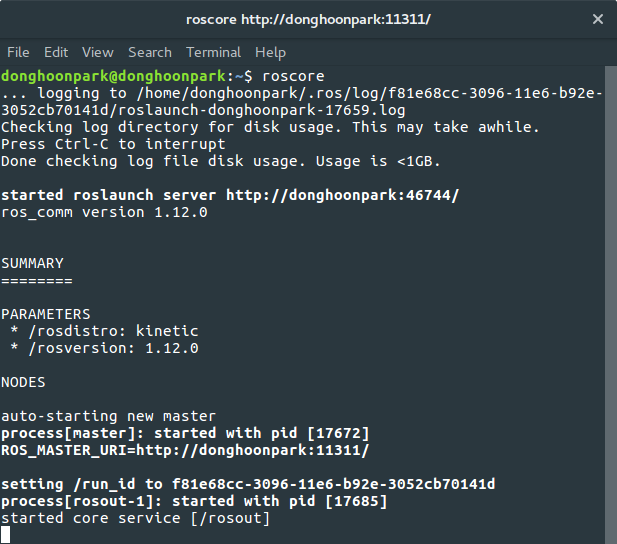
\includegraphics[scale=0.5]{06_roscore_terminal}
\caption{roscore 실행 창}
\end{figure}


%------------------------------------------------
\section{Python Development Environment}\index{Python Development Environment}

이제 프로그래밍 언어인 파이선을 사용하기 위한 개발환경을 갖추어 봅시다.
프로그래밍 언어 개발환경은 크게 세 가지로 구성됩니다. Editor, Compiler, Debugger.
여기에서는 IDE 한 가지를 추천하고, 혹시나 상황이 여의치 않을 경우 사용할 수 있는 오픈소스 개발환경 구축법을 소개하도록 하겠습니다.

\subsection{Pycharm}\index{Pycharm}

\begin{figure}[h]
\centering
\includegraphics[scale=0.5]{07_pycharm}
\caption{pycharm}
\end{figure}

Pycharm은 Jetbrains에서 만든 Python 전용 IDE입니다. 파이선 패키지만 설치된 상태라면 자동으로 모든 설정을 알아서 수행하며, 설치만 하면 바로 사용할 수 있는 상태가 됩니다.
아쉬운 점이라면 다른 환경에 비해 비교적 무겁다는 점과, 무료가 아니라는 점입니다. 그러나 학생인증을 하면 무료로 받을 수 있으므로 학생이라면 해당 IDE를 사용하는 것을 권장합니다.
개인적인 감상으로는 여타 개발 프로그램에 비해 비싼 편이 아니므로 구매하는 것도 상당히 좋은 선택일 것입니다.(필자는 위 회사와 아무런 관련이 없습니다.)
Pycharm은 아래 링크로 가면 다운로드 받을 수 있습니다.

\begin{link}[https://www.jetbrains.com/pycharm/]
  : Pycharm 공식 홈페이지
\end{link}

\begin{figure}[h]
\centering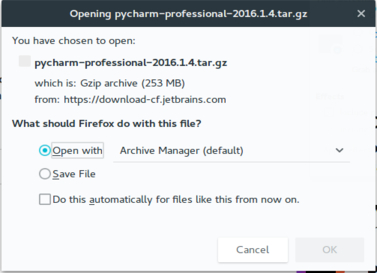
\includegraphics[scale=0.5]{08_pycharm_download}
\caption{pycharm 다운로드}
\end{figure}

Pycharm을 다운로드 받고, 설치하는 방법에 대해 이야기하겠습니다. tar.gz 확장자를 가진 파일은 tar 명령어 혹은 파일 압축풀기 프로그램을 이용해 압축을 해제할 수 있습니다.
압축을 푸는 법은 검색해서 찾아보시고, 압축이 풀린 상태에서 아래 그림과 같이 커멘드라인에서 해당 경로로 이동 후 실행파일을 실행(./) 시켜주면 됩니다.

\begin{figure}[h]
\centering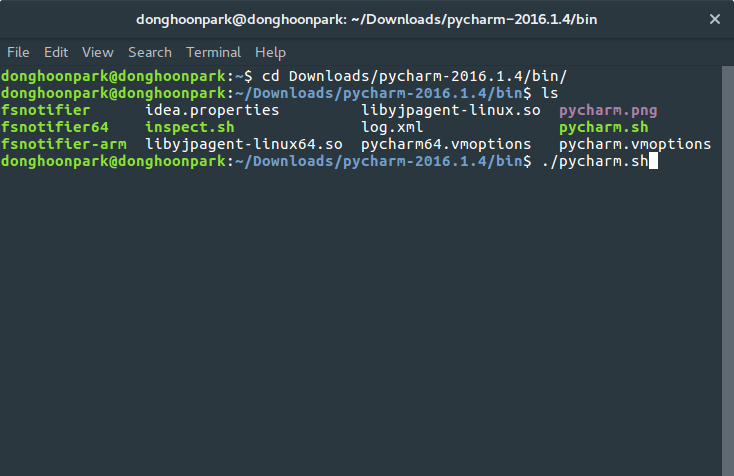
\includegraphics[scale=0.4]{09_pycharm_install}
\caption{pycharm 설치}
\end{figure}

\begin{figure}[h]
\centering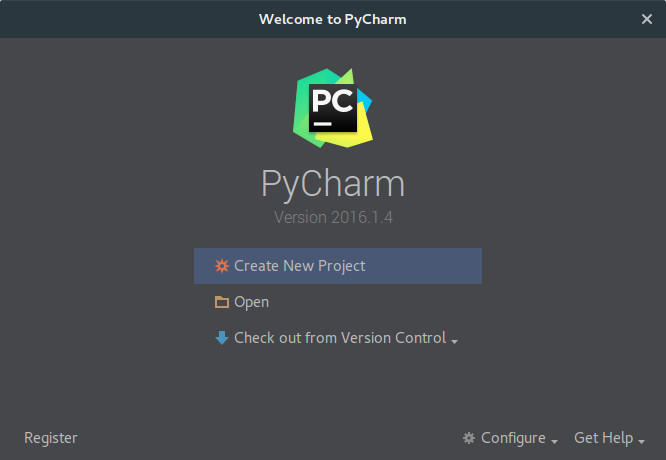
\includegraphics[scale=0.4]{10_pycharm_installed}
\caption{pycharm 실행화면}
\end{figure}

이제 new project를 누르고 프로그래밍을 시작하면 됩니다. Pycharm을 설치했다면 이후 단계를 생략해도 좋습니다.

\subsection{Python Package Install}\index{Python Package Install}

IDE를 사용하지 않는 경우에는 IDE에 해당하는 환경을 각각 구성해줘야 합니다. 각각의 환경이 또 파이선을 사용하는 경우가 많아 파이선 패키지 관리자를 먼저 설치하고 시작하도록 하겠습니다.
아래의 명령어 한 줄이면 Python Package 관리자인 pip이 설치됩니다.

\# sudo apt-get install python-pip

이제 pip에서 아래의 패키지들을 명령줄 도구로 설치해봅시다.

\# sudo pip install jedi

\# sudo pip install pylama

jedi는 파이선 언어 자동완성 패키지이고, pylama는 파이선 언어 코드 형식 및 에러체크 패키지입니다.

\subsection{Atom Editor Install}\index{Atom Editor Install}

이제 에디터를 설치하고 위에서 설치한 파이선 패키지들을 연결해봅시다.

\begin{figure}[h]
\centering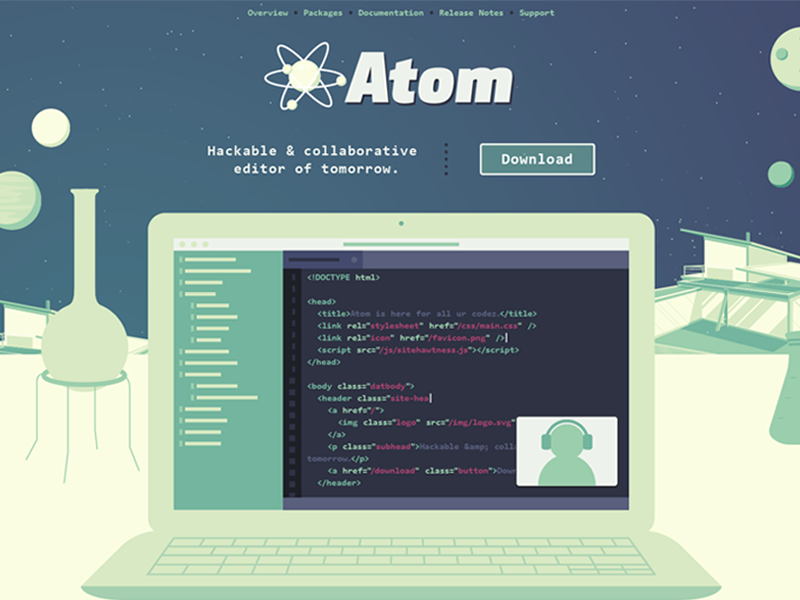
\includegraphics[scale=0.45]{11_atom}
\caption{Atom Editor}
\end{figure}

Atom은 Github에서 만든 에디터로, 상당히 사용자 친화적인 인터페이스를 제공합니다.
물론 속도가 조금 느리다는 평이 있지만, 속도를 중요시하는 분들은 Vim이나 Emacs를 알아서 잘 사용하실 것으로 믿기에 에디터는 Atom 에디터만 다루고 넘어가도록 하겠습니다.
아래 링크로 들어가서 Atom editor 패키지를 받습니다.(.deb)

\begin{link}[https://atom.io/]
  : Atom Editor 공식 홈페이지
\end{link}

.deb 패키지는 실행시키면 소프트웨어 센터에 연결되며 설치가 될 것입니다. 이제 위 파이선 패키지들에 연결할 에디터 패키지를 설치해봅시다.
atom을 실행한 후 Ctrl+, 를 누르면 세팅 메뉴가 열리고, 여기서 새로운 패키지들을 설치할 수 있습니다.

\begin{figure}[h]
\centering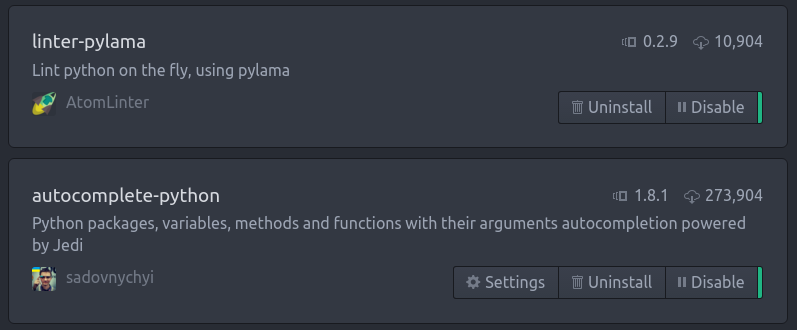
\includegraphics[scale=0.4]{12_atom_packages}
\caption{Atom Install Packages}
\end{figure}

위에 있는 두 패키지를 설치하면 됩니다. 이제 ROS를 손쉽게 사용할 수 있도록 autocomplete-python package를 설정하겠습니다.
그 전에 ROS용 파이선 패키지 설치 경로를 알아야 설정이 가능하므로 아래와 같이 Python 쉘을 실행시켜 ROS 모듈을 위치를 알아냅니다.

\begin{figure}[h]
\centering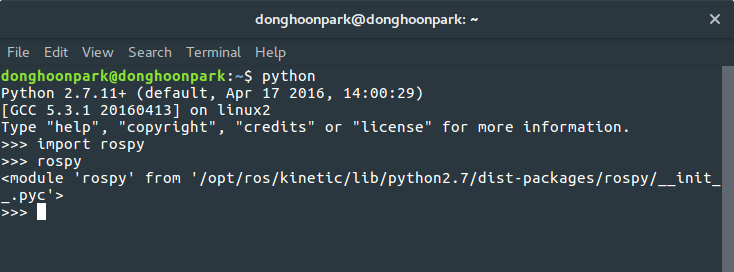
\includegraphics[scale=0.5]{13_ros_module_location}
\caption{ROS 모듈 위치 찾는법}
\end{figure}

아래 창에서 보면 rospy 모듈은 /opt/ros/kinetic/lib/python2.7/dist-packages 에 있는 것을 알 수 있습니다.
해당 경로를 복사해서 jedi 패키지 설정의 Extra Paths for Packages에 넣어줍니다. 그리고 에디터를 재시작한 후 python 파일을 하나 만듭니다.
정상적으로 설치된 경우 아래와 같이 autocompletion과 linter가 잘 작동합니다.

\begin{figure}[h]
\centering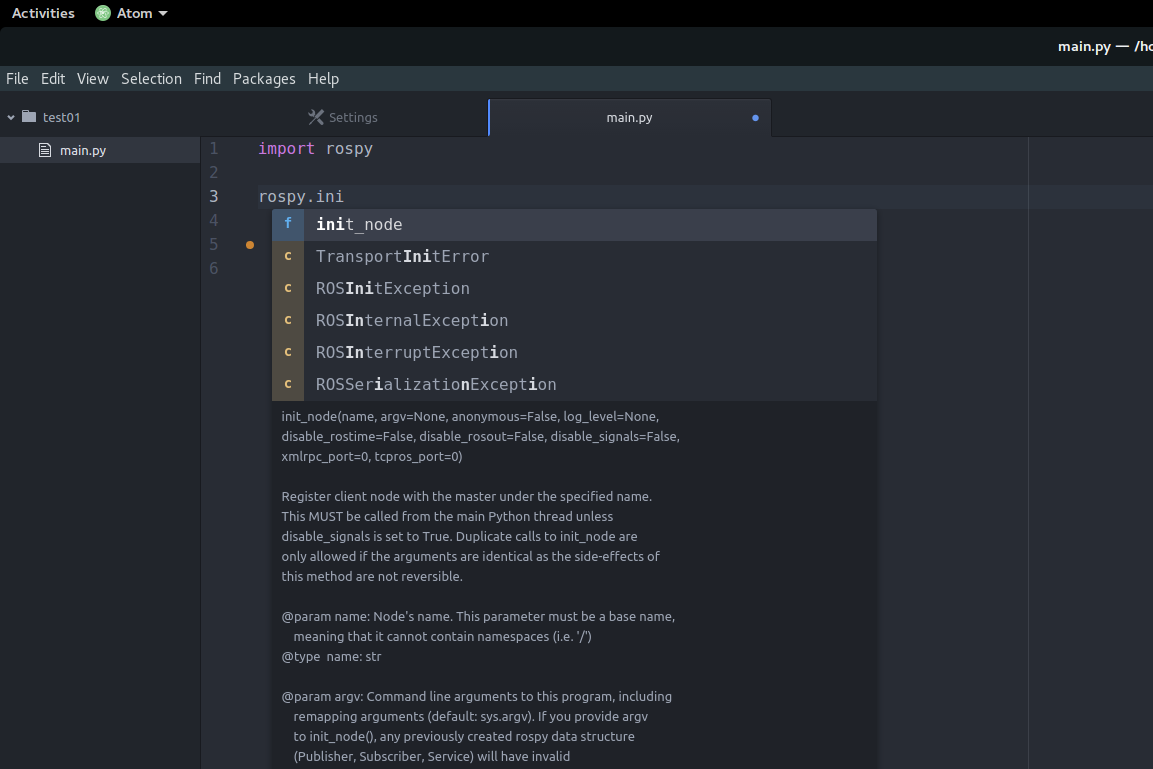
\includegraphics[scale=0.35]{14_atom_setup_complete}
\caption{Atom 정상 실행 상황}
\end{figure}

파이선 개발용 패키지들은 이것 이외에도 유용한 것이 많으니 개인의 취향에 따라 선택해서 더 많은 패키지를 이용해 생산성을 높여보시기 바랍니다.


\section{Matlab Install}\index{Matlab Install}

마지막으로 Matlab을 설치합니다. (학교 혹은 기관 라이선스가 있는 경우에)

\begin{figure}[h]
\centering
\includegraphics[scale=0.7]{15_matlab}
\caption{Matlab}
\end{figure}

Matlab 설치 과정은 Mathworks 사에 매우 자세하게 설명되어있기 때문에 생략하도록 하겠습니다.
ROS 지원 블록을 설치하는 것을 잊지 마세요. 아래 링크를 이용해서 접속하시면 Matlab을 받을 수 있습니다.

\begin{link}[http://kr.mathworks.com/downloads/web\_downloads/?s\_tid=srchtitle   ]
  : Matlab 다운로드 페이지
\end{link}

설치가 완료되면 아래 한 줄 커멘드 라인으로 Matlab 우분투 지원 패키지를 설치하세요. Matlab을 시스템에 알맞게 Integration 시켜주고, 명령줄 상에서 Matlab을 실행할 수 있게 해주는 도구입니다.

\#sudo apt-get install matlab-support

아래와 같이 커맨드라인에서 Matlab을 실행해보는 것으로 Chapter1을 마치겠습니다.

\begin{figure}[h]
\centering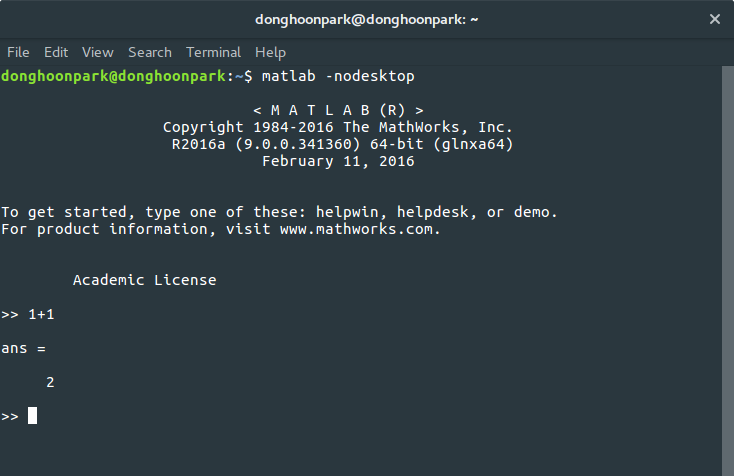
\includegraphics[scale=0.4]{16_matlab_test}
\caption{Matlab Command Line Test}
\end{figure}

%------------------------------------------------

% \section{Citation}\index{Citation}
%
% This statement requires citation \cite{book_key}; this one is more specific \cite[122]{article_key}.
%
% %------------------------------------------------
%
% \section{Lists}\index{Lists}
%
% Lists are useful to present information in a concise and/or ordered way\footnote{Footnote example...}.
%
% \subsection{Numbered List}\index{Lists!Numbered List}
%
% \begin{enumerate}
% \item The first item
% \item The second item
% \item The third item
% \end{enumerate}
%
% \subsection{Bullet Points}\index{Lists!Bullet Points}
%
% \begin{itemize}
% \item The first item
% \item The second item
% \item The third item
% \end{itemize}
%
% \subsection{Descriptions and Definitions}\index{Lists!Descriptions and Definitions}
%
% \begin{description}
% \item[Name] Description
% \item[Word] Definition
% \item[Comment] Elaboration
% \end{description}

%----------------------------------------------------------------------------------------
%	CHAPTER 2
%----------------------------------------------------------------------------------------

\chapter{ROS Topic}

\section{ROS Topic 개요}\index{ROS Topic 개요}

ROS에서 Topic은 비동기로 작동하는 시스템 변수로 볼 수 있습니다. 이 변수를 발행하는 곳(일반적으로 센서)을 Publisher라고 부르고,
이 변수를 받아들이는 곳 (일반적으로 Actuator 등)을 Subscriber라 부르죠. 두 가지 기능을 동시에 하는 경우 (Filter)도 존재할 수 있습니다.
ROS 내용에 대한 보다 개념적인 자세한 설명은 아래 링크의 표윤석 수석연구원님의 책 53p-67p를 참고하기 바랍니다.

\begin{link}[https://github.com/robotpilot/rosbook\_kr/blob/master/pdf/ROS\_Book\_KR.pdf]
  : 로봇 프로그래밍 ROS로 시작하자! - 표윤석 수석연구원님 저
\end{link}

간단한 Line Follower Robot을 ROS로 구성한다고 했을 때 아래 그림과 같이 시스템을 구성해볼 수 있습니다.

\begin{figure}[h]
\centering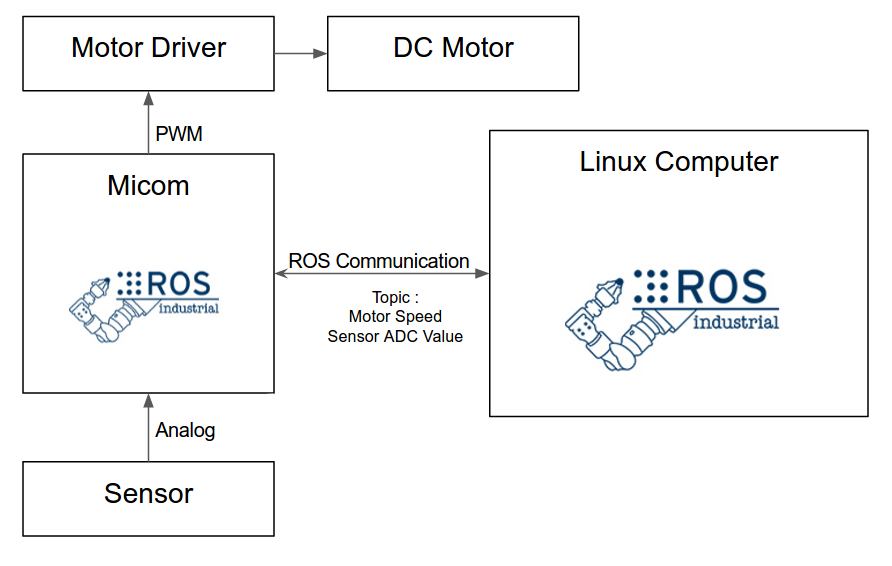
\includegraphics[scale=0.3]{17_ros_system_example}
\caption{ROS System example}
\end{figure}

센서 데이터는 Micom(Arduino, Mbed, STM32 등등)에서 일차적으로 ADC로 읽어오게 됩니다. 그리고 ADC로 읽은 데이터를 ROS에 Publish 하면 ROS 입장에서는 Data가 일정 주기로 계속 업데이트 되는 것으로 보이죠.
모터를 제어할 때도 마찬가지입니다. ROS에서 모터 출력에 대한 변수를 하나 Publish하고, 실제로 모터를 제어하는 Micom이 해당 데이터를 Subscribe하면서 업데이트하면 ROS에서 모터제어를 할 수 있습니다.

\section{Basic Topic Publisher}

\subsection{Rqt를 이용한 Topic Publisher}

시뮬레이션 프로그램을 매우 간단하게 구동해 보면서 Topic을 Publish 한다는 것이 어떤 의미인지 감을 잡아봅시다. ROS는 시뮬레이션 모델에 대한 정보를 Topic으로 불러올 수 있습니다.
해당 Topic들은 시뮬레이션 모델의 물리 벡터를 가지고 있습니다.(Torque, Force 등)
이것들을 Control 하는 방법으로 시뮬레이션을 구동시킬 수 있죠. Topic이 어떤 형태로 나오는지 알아보기 위해서 Gazebo Robot Simulator를 구동해봅시다.
아래의 명령어를 입력하면 Gazebo를 ros에 연결된 상태로 구동할 수 있습니다.

\#rosrun gazebo\_ros gazebo

정상적으로 실행되면 아래와 같은 창을 보실 수 있습니다. 여기에서 컨트롤 할 대상인 Sphere를 하나 불러와 봅시다.

\begin{figure}[h]
\centering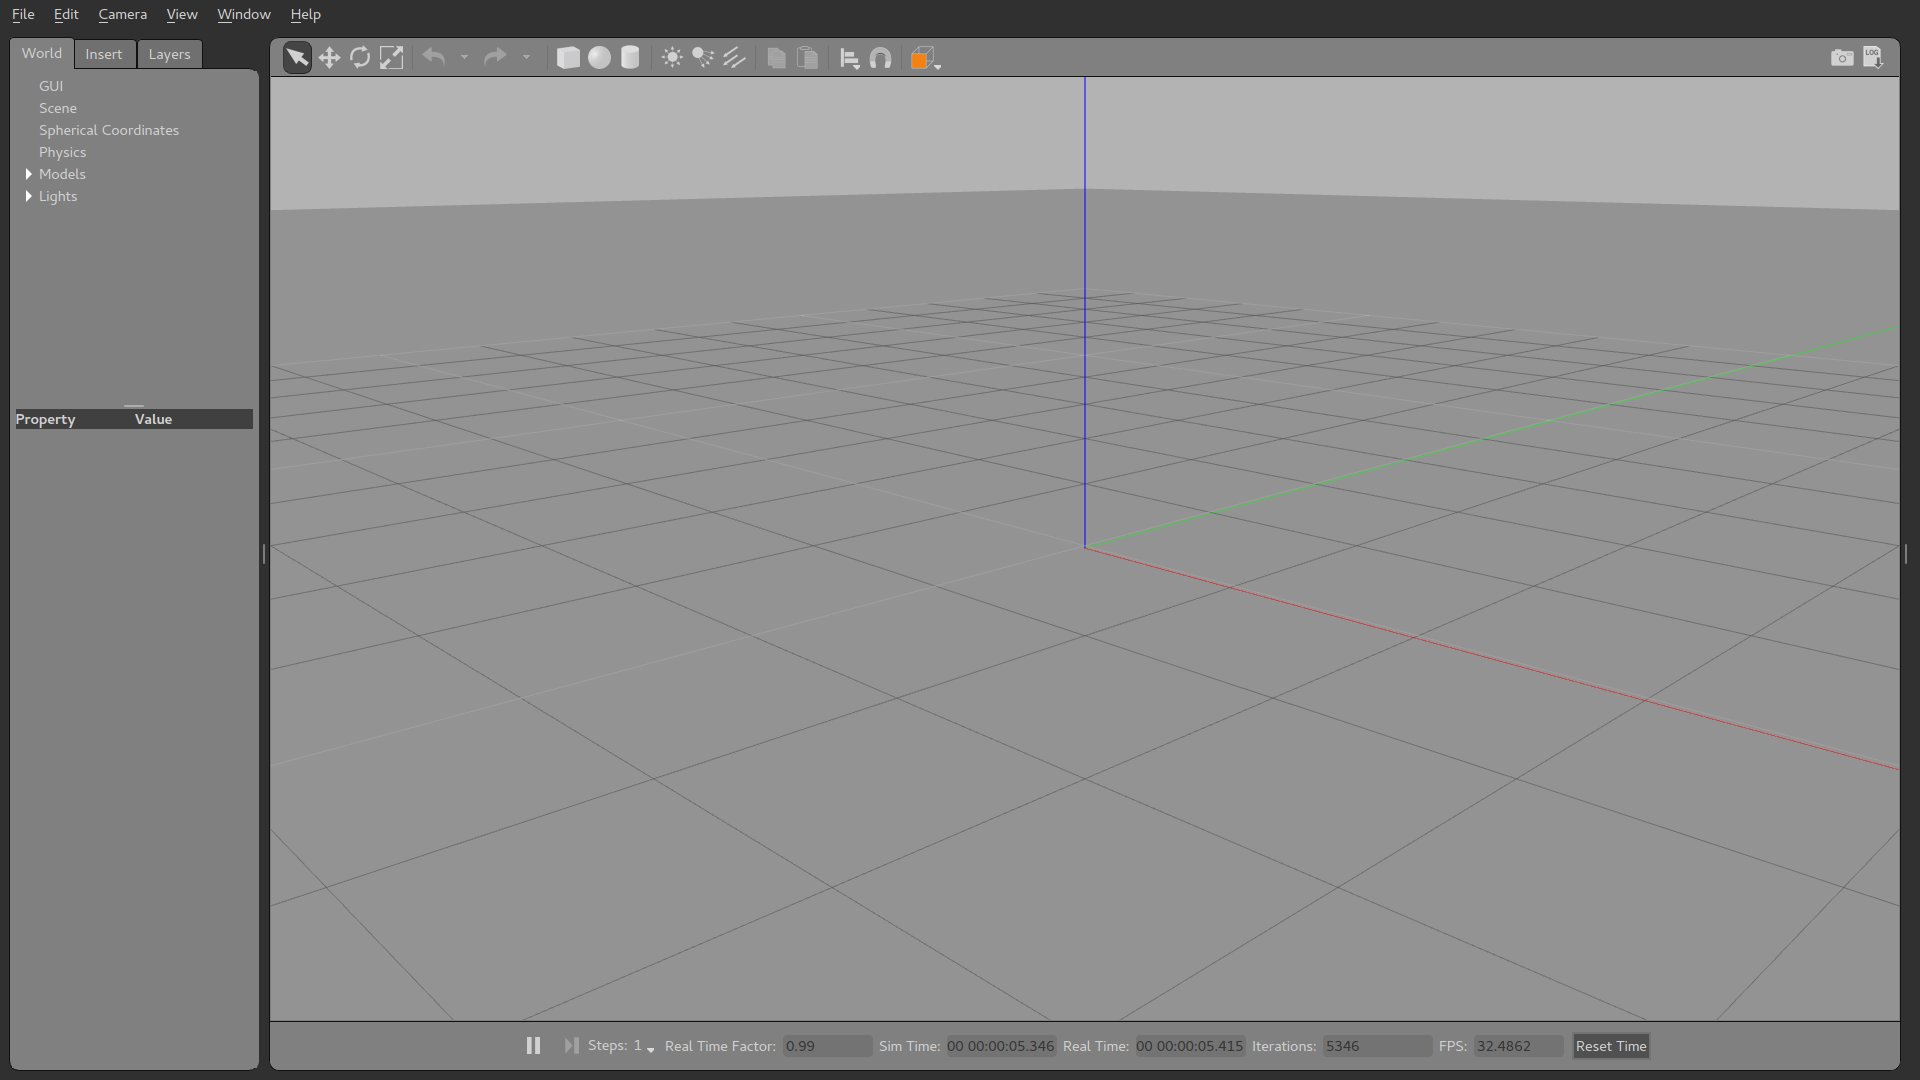
\includegraphics[scale=0.2]{18_gazebo_launch}
\caption{Gazebo 기본 화면}
\end{figure}

gazebo가 정상적으로 구동된 뒤에는 다른 터미널에서 rqt를 구동해봅니다.
rqt에서는 기본 topic publisher를 제공합니다. Plugins -> Topics -> Message Publisher를 열어보세요.

\begin{figure}[h]
\centering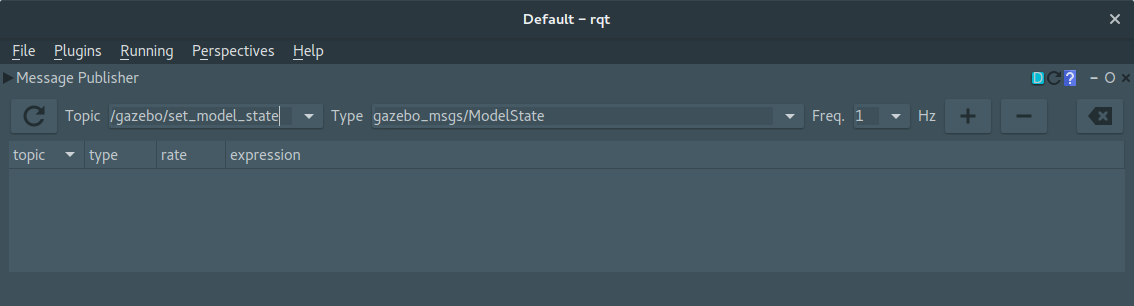
\includegraphics[scale=0.35]{19_rqt_gazebo_topic}
\caption{rqt topic message publisher}
\end{figure}

\#rqt

여기에서 /gazebo/set\_model\_state 라는 topic을 불러와 봅시다. 해당 topic은 Gazebo에서 Subscribe하고 있는 topic으로 해당 내용이 바뀌면
Gazebo는 프로그램에서 해당 모델의 상태를 바꾸어줍니다. 해당 topic을 publish하기 위해서 오른쪽의 \+ 버튼을 눌러 publisher를 추가합니다.
그리고 publish할 message를 아래와 같이 설정합니다. 아래와 같이 설정했을 때 i는 rate가 하나 지날 때 마다 1씩 올라가는 변수이므로, 약 63초마다 원은 원점을 따라서 한 바퀴씩 움직이게 될 것입니다.

\begin{figure}[h]
\centering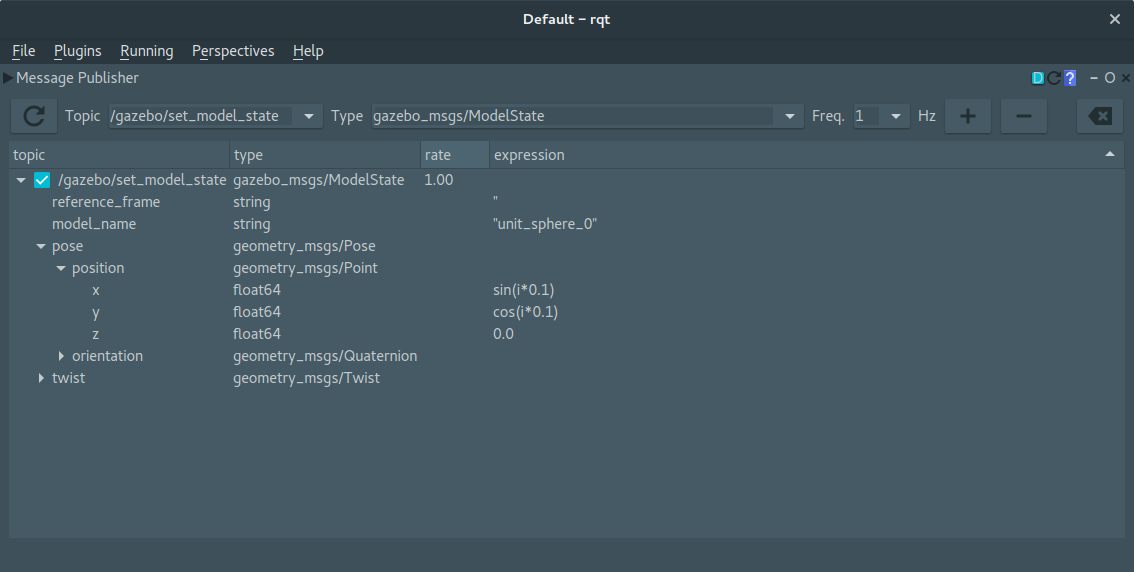
\includegraphics[scale=0.35]{20_rqt_gazebo_topic_pub}
\caption{rqt topic message publisher}
\end{figure}

rqt는 topic 제어 이외에도 여러 기능을 가지고 있기 때문에 간단히 훑어보시는 것도 좋을 것입니다.
특히, Matlab을 사용하지 않는 경우 rqt의 plot 기능은 매우 유용하게 사용할 수 있습니다.

\subsection{Python을 이용한 Topic Publisher}

아래와 같이 파이선 프로그램을 따라서 작성해봅시다.

\begin{minted}[linenos ,numberblanklines=false]{python}
  import rospy
  from std_msgs.msg import String

  rospy.init_node('helloworldnode')

  pub_test = rospy.Publisher('iterator', String, queue_size=10)

  rate = rospy.Rate(10)

  i = 0

  while not rospy.is_shutdown():
      pub_test.publish("hello "+str(i))
      i = i + 1
      rate.sleep()

\end{minted}

코드를 분석하면서 각각이 어떤 부분인지 알아보도록 하죠.

\begin{minted}[linenos,numberblanklines=false]{python}
  import rospy
  from std_msgs.msg import String

\end{minted}

파이선 ROS 패키지들을 가져오는 부분입니다. 파이선은 자료형을 구분하지 않고 사용하지만, ROS의 Topic은 자료형을 꼭 지정해야 합니다.
그래서 String 메세지 패키지를 가져와서 사용하는 것입니다. 이번에 만들 Publisher가 Publish 하는 Topic은 String 형입니다.

\begin{minted}[linenos, firstnumber=last, numberblanklines=false]{python}

  rospy.init_node('helloworldnode')

  pub_test = rospy.Publisher('iterator', String, queue_size=10)

  rate = rospy.Rate(10)
\end{minted}

3행에서는 ROS 노드(ROS 프로그램의 단위)를 initialize 합니다. 이 프로그램을 ROS 상에서 helloworldnode라는 이름으로 불리게 됩니다.
4행에서는 pub\_test 라는 Publisher 객체를 선언합니다. 이 topic Publisher의 이름은 iterator이고, String 형식의 메세지를 Publish하며, Queue Size 는 10입니다.
5행에서는 이 노드가 동작하는 Frequency를 정하고 있습니다. 이 노드는 뒤에 나온 것과 같이 while문을 구성해주면, 초당 10번 불리게 됩니다.

\begin{minted}[linenos, firstnumber=last, numberblanklines=false]{python}

  i = 0

  while not rospy.is_shutdown():
      pub_test.publish("hello "+str(i))
      i = i + 1
      rate.sleep()
\end{minted}

6행에서는 i 변수를 만듭니다.
7행에서는 ROS가 동작하고 있는 한 지속적으로 루프를 돌게되는 무한루프 문을 만듭니다.
8행에서는 publish가 이루어집니다. publish 함수는 해당 topic의 데이터에 해당하는 부분을 input으로 받습니다.
9행에서는 i 변수를 증가시킵니다.

이 파이선 프로그램을 아래 커멘드 라인 명령어를 이용해 실행시킵니다. (python\_file\_path 와 python\_file\_name은 각자 파이선 파일을 만든 경로와 이름에 따라 다를 것입니다.)

\begin{minted}{bash}
  python /python_file_path/python_file_name.py
\end{minted}

에러가 나오지 않는다면 다른 터미널 창을 켜고 아래 명령어를 입력합니다.

\begin{minted}{bash}
  rostopic echo /iterator
\end{minted}

\begin{figure}[h]
\centering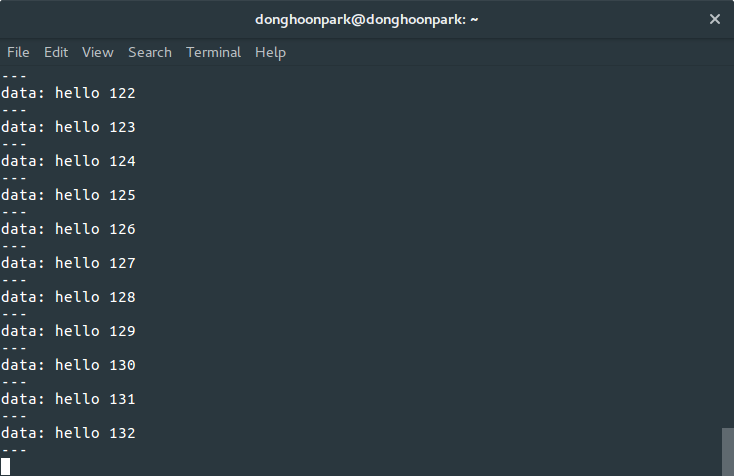
\includegraphics[scale=0.28]{21_topic_echo}
\caption{rostopic echo}
\end{figure}

위와 같이 초당 10번의 메세지가 출력되면 성공입니다. 다른 종류의 Topic에 대해 Publish하고 싶다면 해당 Topic의 자료형에 맞는 형태를 들고와야 합니다.
예를 들어 앞서 rqt에서 했던 Gazebo set\_model\_state Topic의 경우에는 자료형이 ModelState이기 때문에 해당 자료형을 들고와서 사용해주어야 합니다.
예를 들면, rqt에서 했던 것과 같은 작업을 하는 python 코드는 아래와 같습니다.

\begin{minted}[linenos=true, numberblanklines=false]{python}
  import rospy
  import numpy as np
  from gazebo_msgs.msg import ModelState

  rospy.init_node('gazebo_example_node')
  ms = ModelState()

  pub_test = rospy.Publisher('/gazebo/set_model_state', ModelState, queue_size=10)

  rate = rospy.Rate(1)

  i = 0

  while not rospy.is_shutdown():
      ms.model_name = 'unit_sphere_0'
      ms.pose.position.x = np.sin(i * 0.1)
      ms.pose.position.y = np.cos(i * 0.1)
      pub_test.publish(ms)
      i = i + 1
      rate.sleep()

\end{minted}

\subsection{Arduino를 이용한 Topic Publisher}

이번엔 하드웨어에서 Topic을 불러들여오는 작업을 해보겠습니다.
가장 보편적으로 쓰이는 Micom인 아두이노를 이용해서 ROS Topic을 Publish하는 방법에 대해 이야기하겠습니다.
아래 사진과 같이 아두이노를 구성하고, 컴퓨터와 연결해주세요.

\begin{figure}[h]
\centering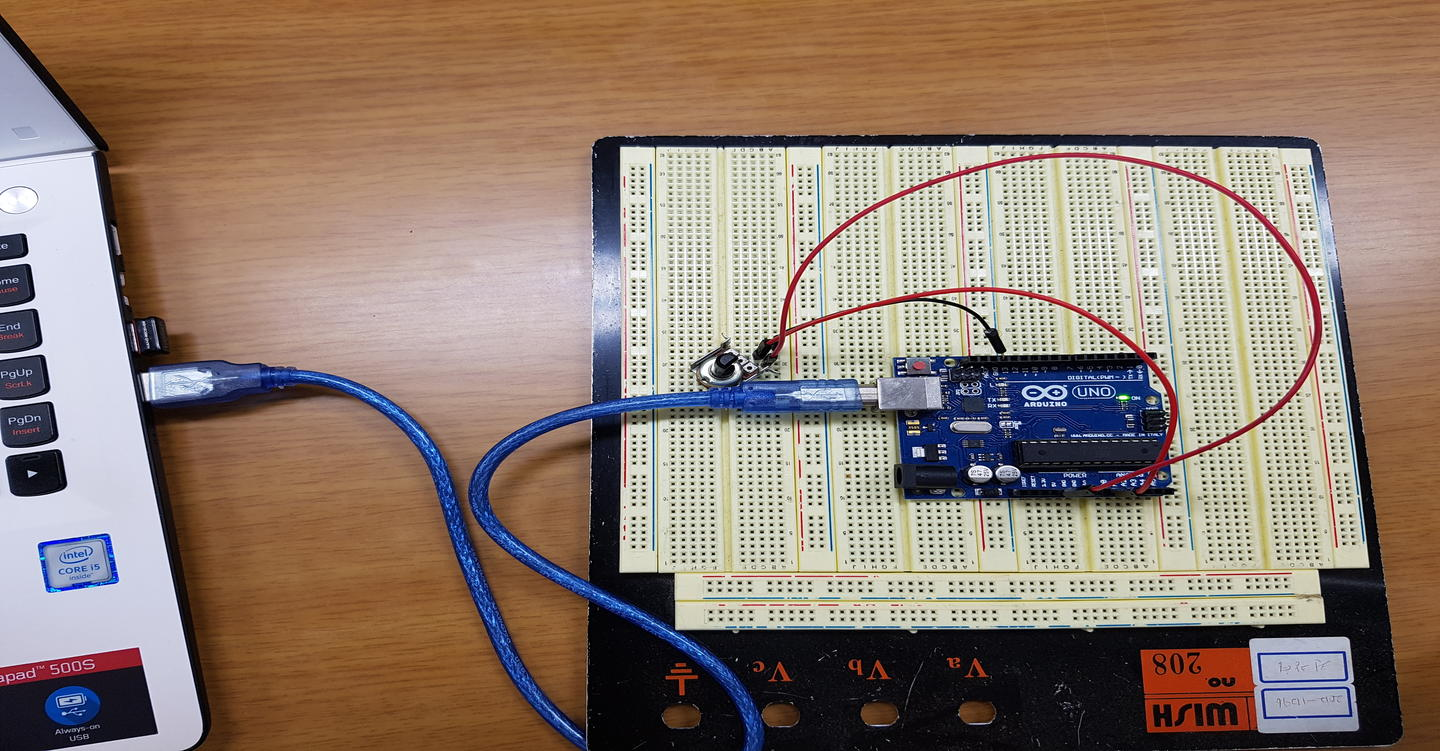
\includegraphics[scale=0.28]{22_arduino_connect}
\caption{rostopic echo}
\end{figure}

+5V <-> POT1

A0 <-> POT2

GND <-> POT3

위와 같이 연결해주면 됩니다. 아두이노와 컴퓨터를 ROS로 연결하기 위해서는 rosserial이라는 패키지를 설치해야 합니다.
2016.06 기준 Kinetic에서는 apt-get 패키지로 rosserial이 지원되지 않기 때문에 catkin 빌드 과정을 거쳐야 합니다.
indigo, jade 사용자라면 아래와 같이 입력하면 간단하게 rosserial package가 설치됩니다.

\begin{minted}{bash}
  sudo apt-get install ros-indigo-rosserial  (indigo)
  sudo apt-get install ros-jade-rosserial  (jade)
\end{minted}

kinetic 사용자라면, catkin 빌드 과정을 거쳐야 하는데, 패키지 설치 연습을 해보기 위해 jade, indigo 사용자분들도 따라해보시길 권장합니다.
먼저 아래 링크로 이동해서 패키지의 remote 저장소 주소를 가져옵니다.

\begin{link}[https://github.com/ros-drivers/rosserial]
  : rosserial git 저장소
\end{link}

그리고 아래와 같이 catkin\_workspace를 생성하고 저장소 주소를 통해 소스를 가져옵니다.
괄호 안의 내용은 설명이므로 입력하지 마세요.

\begin{minted}{bash}
  cd (홈 디렉토리로 이동)
  mkdir catkin_workspace (catkin workspace 폴더 생성)
  cd catkin_workspace (catkin workspace 폴더로 이동)
  mkdir src (소스 폴더 생성)
  cd src (소스 폴더로 이동)
  git clone https://github.com/ros-drivers/rosserial.git (rosserial 저장소 가져오기)
\end{minted}

clone이 끝나면 상위 디렉토리로 이동해서 catkin 패키지를 빌드합니다.

\begin{minted}{bash}
  cd .. (catkin workspace 폴더로 이동)
  catkin_make (catkin 빌드)
  catkin_make install (빌드된 패키지들 인스톨)
\end{minted}

그리고 리눅스 쉘 명령어 집합인 bash(zsh을 쓰는 분이면 뒤의 과정을 전부 zsh로 진행하시면 됩니다.)에 새로 인스톨한 패키지를 등록하기 위해서는 아래와 같은 과정을 수행해야 합니다.
catkin\_workspace 안쪽의 install 폴더가 생성되어있을텐데, 여기에 있는 setup.bash file을 실행해주어야 해당 터미널에서 새로 설치한 패키지들을 사용할 수 있습니다.
그러나 터미널을 켤 때마다 이것을 실행시키는 것은 매우 귀찮은 일이죠. 그래서 자동으로 터미널이 처음 로드될 때마다 해당 bash file이 실행되도록 설정해봅시다.
아래 명령어를 이용해서 bash 설정파일인 .bashrc를 열어서 수정해봅시다.

\begin{minted}{bash}
  cd
  gedit .bashrc
\end{minted}

아래와 같은 창이 열리는데, 가장 아래로 이동해보시면, ROS를 제대로 설치하셨다는 가정 하에 한 줄의 코드가 있을 것입니다.

\begin{minted}{bash}
  source /opt/ros/kinetic/setup.bash
\end{minted}

이 코드는 bash를 실행할 때 저 경로에 있는 setup.bash 파일을 실행한다는 뜻입니다.
이번엔 catkin workspace의 install 폴더의 setup.bash를 실행시켜야 하므로 아래와 같이 코드를 한 줄 넣어주면 됩니다.

\begin{minted}{bash}
  source ~/catkin_workspace/install/setup.bash
  source ~/catkin_workspace/devel/setup.bash
\end{minted}

새로운 터미널을 켜고, rospack 명령어를 통해 ros 패키지가 정상적으로 설치되었는지 확인해봅시다.

\begin{minted}{bash}
  rospack list
\end{minted}

rosserial은 리눅스 컴퓨터에 설치된 Main ROS와 외부 하드웨어 ROS 노드를 Serial 통신으로 연결합니다.
그러면 외부 ROS 노드 또한 ROS 라이브러리를 불러와서 작성해주고, 코드를 넣어주어야겠죠. 아두이노는 기본으로
ROS 라이브러리를 포함하고 있지 않기에 라이브러리를 설치해주어야 합니다.
아두이노 설치폴더로 이동한 뒤 아래와 같은 명령어를 입력해서 ROS Serial 라이브러리를 설치합니다.

\begin{minted}{bash}
  cd libraries
  rosrun rosserial_arduino make_libraries.py .
\end{minted}

라이브러리 설치 후 아래 코드를 컴파일해서 아두이노에 넣어봅시다. 혹시나 SerialPort Permission 때문에 코드 업로드가 되지 않는다면 아래 명령어를 입력하세요.

\begin{minted}{bash}
  sudo chmod 666 /serial/port/location
  ex) sudo chmod 666 /dev/ttyACM0
\end{minted}

\begin{minted}[linenos ,numberblanklines=false]{cpp}
  #include <ros.h>
  #include <std_msgs/Int16.h>


  ros::NodeHandle nh;

  std_msgs::Int16 adc_msg;
  ros::Publisher adc_publisher("adc_publisher", &adc_msg);

  const int adc_pin = A0;

  void setup()
  {
    nh.initNode();
    nh.advertise(adc_publisher);

    pinMode(adc_pin, INPUT);

  }

  void loop()
  {
    adc_msg.data = analogRead(A0);
    adc_publisher.publish(&adc_msg);
    nh.spinOnce();
    delay(50);
  }
\end{minted}

위의 코드는 아두이노에서 A0핀의 ADC 값을 읽은 뒤 50ms 주기로 데이터를 보내주는 코드입니다.
코드 내용을 나누어서 분석해봅시다.

\begin{minted}[linenos ,numberblanklines=false]{cpp}
  #include <ros.h>
  #include <std_msgs/Int16.h>
\end{minted}

ros header file을 가져옵니다. Int16 형식의 Topic을 해석하고 보내기 위한 헤더 또한 가져옵니다.

\begin{minted}[linenos, firstnumber=last ,numberblanklines=false]{cpp}
  ros::NodeHandle nh;

  std_msgs::Int16 adc_msg;
  ros::Publisher adc_publisher("adc_publisher", &adc_msg);
\end{minted}

3행에서는 ROS의 node를 설정하기 위한 객체를 선언하고
4행에서는 Int16 형식의 메세지를 선언합니다.
5행에서는 Publisher를 선언하고, 해당 Publisher가 받을 메세지 객체를 포인터로 넘겨줍니다.

\begin{minted}[linenos, firstnumber=last ,numberblanklines=false]{cpp}
  const int adc_pin = A0;

  void setup()
  {
    nh.initNode();
    nh.advertise(adc_publisher);

    pinMode(adc_pin, INPUT);

  }
\end{minted}

6행에서는 하드웨어에서 adc\_pin 을 A0 핀으로 정의합니다.
9행에서는 ROS node를 초기화합니다.
10행에서는 노드에서 해당 publisher를 등록합니다.
11행에서는 하드웨어 adc\_pin 을 input으로 정의합니다.

\begin{minted}[linenos, firstnumber=last ,numberblanklines=false]{cpp}
  void loop()
  {
    adc_msg.data = analogRead(A0);
    adc_publisher.publish(&adc_msg);
    nh.spinOnce();
    delay(50);
  }
\end{minted}

15행에서는 adc\_msg의 data를 A0핀에서 읽어온 ADC 값으로 채워넣습니다.
16행에서는 publisher가 topic을 publish합니다.
17행에서 spinOnce 함수를 불러오며 실제 데이터 교환이 일어납니다.
18행에서 1/20 초 딜레이를 줍니다.

코드를 아두이노에 올린 뒤에는 아래 명령어를 통해 컴퓨터와 아두이노를 연결하세요. 아두이노의 시리얼 포트를 잘 기억하고 있으셔야 합니다.
터미널에 아래와 같이 명령어를 입력해서 rosserial\_python package를 실행하세요. 잠시 기다리면 아두이노와 통신을 시작합니다.
만약 시리얼포트 번호가 /dev/ttyACM0가 아니라면 아래의 포트 번호를 자신의 시스템에 맞는 번호로 바꾸어주세요.

\begin{minted}{bash}
  rosrun rosserial_python serial_node.py /dev/ttyACM0
\end{minted}

아래 터미널 창과 같이 rosserial 창이 실행되면 성공입니다. rosserial로 연결된 뒤에는 어떤 topic이 rosserial을 통해 공유되고 있는지에 대한 정보가 같이 들어옵니다.
이제 해당 topic은 ROS에서 python, Matlab 등의 언어를 이용해여 subscribe가 가능합니다.
하지만 주의해야 하는 점은 rosserial은 serial 통신이라는 상대적으로 저속의 통신으로 연결되기 때문에 생각보다 많은 topic을 실시간으로 공유하지는 못합니다.
topic이 많아진다면 slave 하드웨어 (아두이노 등)을 더 좋은 성능의 것으로 업그레이드 하는 것을 추천합니다.

\begin{figure}[h]
\centering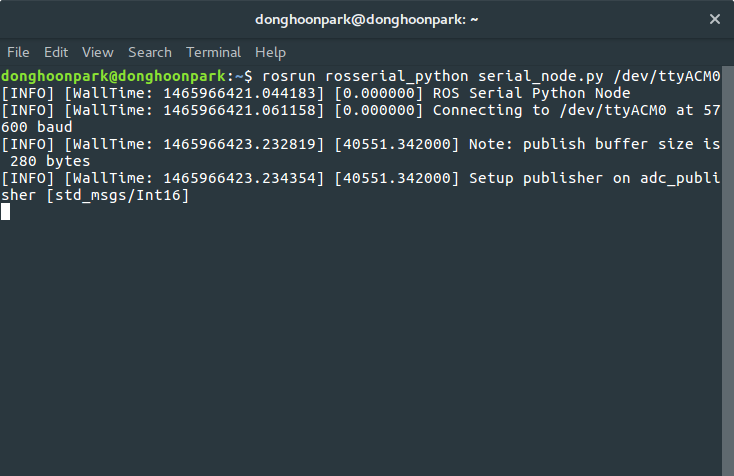
\includegraphics[scale=0.28]{23_rosserial_run}
\caption{rostopic echo}
\end{figure}

이제 rqt로 Publish 된 데이터를 확인해봅시다. rqt의 matplot을 이용하면 아래와 같이 데이터를 뽑아서 볼 수 있습니다.

\begin{figure}[h]
\centering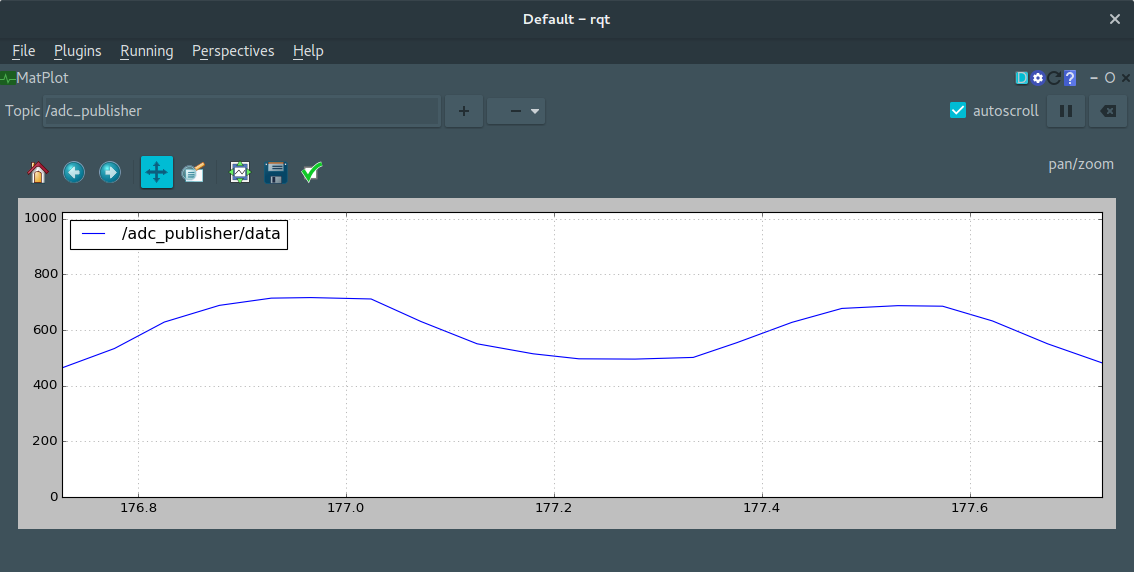
\includegraphics[scale=0.28]{24_rqt_matplot}
\caption{rostopic echo}
\end{figure}

\section{Basic Topic Subscriber}

이제는 여러 가지 환경에서 Topic을 Subscribe하는 방법에 대해 알아보도록 하겠습니다. Subscribe는 Publish된 Topic을 가져오는 것으로, 가져온 데이터를 이용해 프로그램의 동작을 결정하거나 할 수 있습니다.
앞서 소개한 커맨드라인 도구인 rostopic echo 또한 topic subscribe를 하는 프로그램 중 하나입니다.
이번 단원 역시 rqt, Python, Arduino 등을 이용해서 Topic을 제어하는 연습을 해보도록 하겠습니다.
하나 더 추가해서, Matlab Simulink를 이용한 Topic 제어 또한 이야기할테니 차근차근 따라와 주세요.

\subsection{rqt를 이용한 Topic Subscribe}

subscribe할 Topic을 뽑아주는 Publish node로 사용하기 위해서
앞서 작성한 Gazebo에 Topic을 Publish하는 Python ROS node를 실행시킵니다.
그리고 rqt를 실행시키고 Topic 모니터를 켜면 아래와 같은 화면을 볼 수 있습니다.
Topic에 대한 정보가 완전히 표시되는 것을 확인할 수 있으며, 업데이트 또한 실시간으로 됩니다.
단순한 모니터링 용도라면 rqt를 이용해서 Topic을 보는 것이 가장 효율적입니다.

\begin{figure}[h]
\centering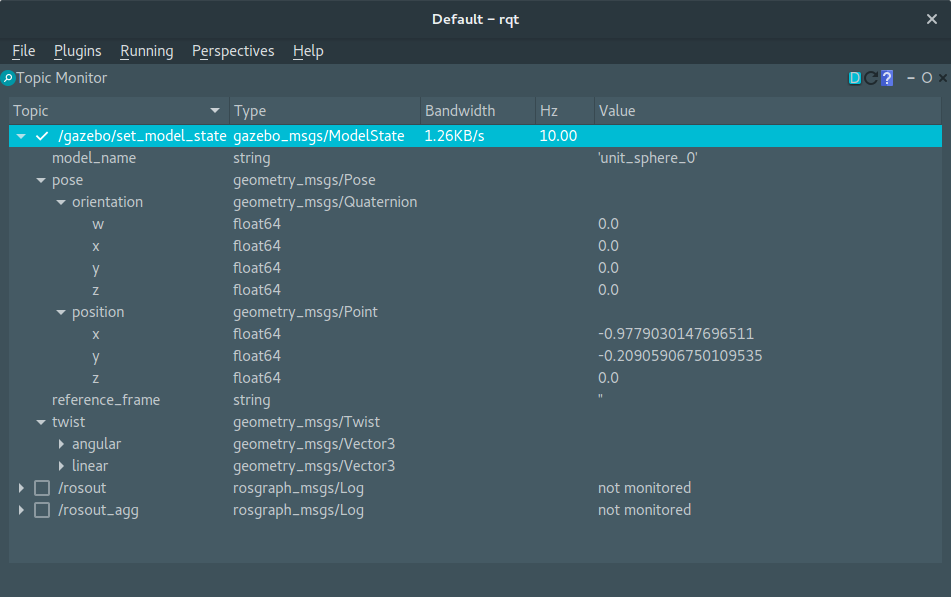
\includegraphics[scale=0.4]{25_rqt_subscribe}
\caption{rqt Topic Mointor}
\end{figure}

\subsection{Python을 이용한 Topic Subscribe}

아래와 같이 파이선 프로그램을 작성해봅시다. 해당 파이선 프로그램은 chatter라는 이름의 topic을 읽어와서 그 데이터를 출력해주는 프로그램입니다.


\begin{minted}[linenos ,numberblanklines=false]{Python}
  import rospy
  from std_msgs.msg import String


  def chatterCallback(chatter):
      rospy.loginfo(chatter.data)


  def listener():
      rospy.init_node('chatter_node')
      rospy.Subscriber("chatter", String, chatterCallback)
      rospy.spin()

  if __name__ == '__main__':
      listener()
\end{minted}

앞서 Topic Publish에서 했던 내용들도 많이 있는데, 이번에도 부분부분 나누어 설명을 해보도록 하겠습니다.

\begin{minted}[linenos , numberblanklines=false]{Python}
  import rospy
  from std_msgs.msg import String
\end{minted}

rospy 패키지와 standard message 패키지를 불러옵니다.

\begin{minted}[linenos, firstnumber=last, numberblanklines=false]{Python}

  def chatterCallback(chatter):
      rospy.loginfo(chatter.data)

\end{minted}

chatterCallback이라는 이름의 callback 함수를 정의합니다. callback 함수란 특정 상황에서 불리도록 설정된 함수로,
사용자 입장에서는 이벤트 함수와 비슷한 개념이라고 보시면 됩니다.
해당 함수는 Subscribe 하고 있는 topic에 대한 데이터가 들어왔을 때 불리는 callback 함수로 지정될 것입니다.
callback이 일어나고 나면 해당 함수는 subscribe하는 topic을 객체로 들고옵니다. 그 객체가 callback 함수의 parameter로, 여기에서는 chatter 객체입니다.
결론적으론 해당 객제의 data를 log 함수에 넣어서 ros에서 데이터 로그를 찍게 하는거죠.

\begin{minted}[linenos, firstnumber=last, numberblanklines=false]{Python}

  def listener():
      rospy.init_node('chatter_node')
      rospy.Subscriber("chatter", String, chatterCallback)
      rospy.spin()

\end{minted}

6행에서 노드 초기화, 7행에서 Subscriber 설정 및 callback 함수 지정이 이루어집니다.
8행에서는 spin 함수를 이용해서 노드가 roscore가 죽지 않는 이상 계속 동작하도록 만듭니다.

\begin{minted}[linenos, firstnumber=last, numberblanklines=false]{Python}

  if __name__ == '__main__':
      listener()

\end{minted}

listener 함수를 실행시킵니다.

이제 해당 파이선 파일을 실행시키고, rqt에서 무언가 chatter topic을 아래와 같이 publish 해봅시다.

\begin{figure}[h]
\centering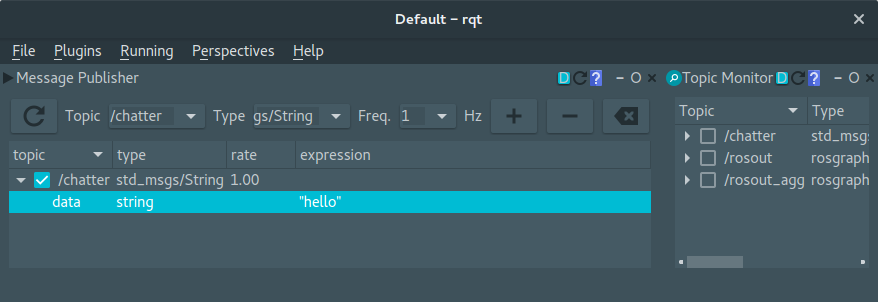
\includegraphics[scale=0.4]{26_rqt_publisher}
\caption{rqt hello publisher}
\end{figure}

파이선 프로그램을 연 터미널에서는 아래와 같이 1초마다 로그를 전송할 것입니다.

\begin{figure}[h]
\centering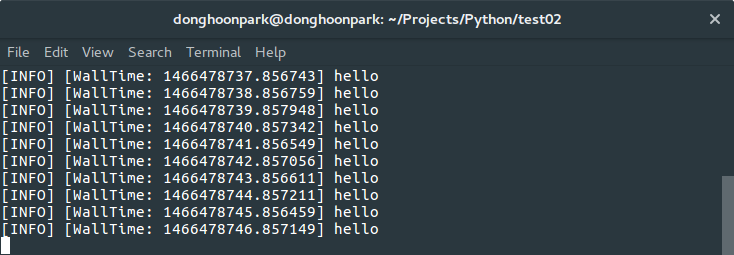
\includegraphics[scale=0.4]{27_python_subscriber}
\caption{python subscriber example}
\end{figure}

\subsection{Arduino를 이용한 Topic Subscribe}

Topic Subscriber를 작성하기 위해 아두이노 하드웨어를 아래 사진과 같이 구성해봅시다.

아래와 같이 프로그램을 짜봅시다. 해당 프로그램은 ros 예제에도 수록되어 있습니다.

\begin{minted}[linenos, numberblanklines=false]{cpp}

#include <Servo.h>
#include <ros.h>
#include <std_msgs/UInt16.h>

ros::NodeHandle  nh;

Servo servo;

void servo_cb( const std_msgs::UInt16& cmd_msg){
  servo.write(cmd_msg.data); //set servo angle, should be from 0-180
  digitalWrite(13, HIGH-digitalRead(13));  //toggle led
}


ros::Subscriber<std_msgs::UInt16> sub("servo", servo_cb);

void setup(){
  pinMode(13, OUTPUT);

  nh.initNode();
  nh.subscribe(sub);

  servo.attach(9); //attach it to pin 9
}

void loop(){
  nh.spinOnce();
  delay(1);
}
ce();
  delay(1);
\end{minted}

지금까지와 같이 부분별로 분석해봅시다.

\begin{minted}[linenos, numberblanklines=false]{cpp}

#include <Servo.h>
#include <ros.h>
#include <std_msgs/UInt16.h>

\end{minted}

서보모터 컨트롤, ROS, standard message 라이브러리를 불러옵니다.

\begin{minted}[linenos, firstnumber=last, numberblanklines=false]{cpp}
  ros::NodeHandle  nh;

  Servo servo;
\end{minted}

ros node와 서보모터 객체를 선언합니다.

\begin{minted}[linenos, firstnumber=last, numberblanklines=false]{cpp}
  void servo_cb( const std_msgs::UInt16& cmd_msg){
    servo.write(cmd_msg.data); //set servo angle, should be from 0-180
    digitalWrite(13, HIGH-digitalRead(13));  //toggle led
  }
\end{minted}

서보모터 subscriber에 대한 callback 함수를 만듭니다.
6행에서 보면 이 callback 함수는 standard message의 UInt16 type message를 parameter로 받습니다.
그리고 7행에서 보면 해당 메세지 데이터를 servo 객체에 써 넣어줍니다.

\begin{minted}[linenos, firstnumber=last, numberblanklines=false]{cpp}
  ros::Subscriber<std_msgs::UInt16> sub("servo", servo_cb);
\end{minted}

ROS Subscriber 객체를 선언하고, 해당 객체를 servo 라는 이름의 topic과 연결합니다. 그리고 해당 Subscriber의 Callback 함수로 servo\_cb를 지정합니다.

\begin{minted}[linenos, firstnumber=last, numberblanklines=false]{cpp}
  void setup(){
    pinMode(13, OUTPUT);

    nh.initNode();
    nh.subscribe(sub);

    servo.attach(9); //attach it to pin 9
  }
\end{minted}

setup과정을 수행합니다. 13행에서 node를 초기화하고, 14행에서 subscribe 객체를 node에 연결합니다.
15행에서 9번 핀에 연결되는 서보를 초기화합니다.

\begin{minted}[linenos, firstnumber=last, numberblanklines=false]{cpp}
  void loop(){
    nh.spinOnce();
    delay(1);
  }
\end{minted}

spinOnce 함수를 호출하면서 실제로 rosserial\_py 와 통신이 이루어집니다. 그 뒤 1ms의 딜레이를 가지고,
spinOnce 작업을 반복적으로 수행합니다.

rqt를 이용해서 실제로 서보모터를 ROS로 구동해봅시다. 아래와 같이 topic publisher를 설정한 뒤 실행시키면 서보모터가 3초 주기로 sweep 하는 것을 볼 수 있습니다.
% i는 rqt에서 Publish할 때마다 1씩 증가하는 함수로, 아래와 같이 rqt설정을 했을 시에는 초당 100씩 증가하는 변수로 생각하면 됩니다.

\begin{figure}[h]
\centering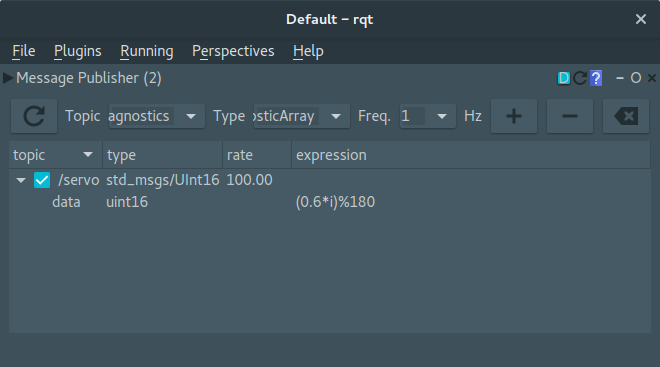
\includegraphics[scale=0.4]{28_rqt_servo}
\caption{rqt servo example}
\end{figure}

\section{Topic Publisher \& Subscriber 응용}

\subsection{Matlab Simulink를 이용한 Topic 제어}

Matlab은 많은 엔지니어가 사용하는 플랫폼으로, 여러 공학적 프리셋들을 매우 신뢰도 있게 제공해줍니다. 특히 신호처리에서는 Matlab보다 나은 플랫폼을 찾기 어려운 정도인데요,
놀랍게도 Matlab도 ROS 연동이 가능합니다. 심지어 매우 잘 됩니다. 그래서 이번 단원에서는 Matlab을 어떻게 ROS와 연동시키는지에 대해 이야기하고자 합니다.
Matlab ROS 연동은 아래 페이지에 공식 튜토리얼이 나와있습니다. 순서대로 따라 해 보실 수 있습니다.
Matlab 코드를 그냥 사용하는 것은 매우 느리기 때문에, Matlab Coder를 꼭 이용해서 컴파일 후 사용하는 것을 권장합니다.
아래 튜토리얼 중 Generate a standalone ROS node from Simulink 를 참고하시면 됩니다.
Matlab Coder가 Node가 들어있는 패키지 형태로 Matlab Simulink model을 만들어줍니다.

\begin{link}[http://kr.mathworks.com/help/robotics/examples.html]
  : Matlab ROS Tutorial
\end{link}

공식 튜토리얼이 있고, Matlab 라이선스 문제로 인해 교재에 내용을 더 넣지는 않겠습니다.


\subsection{ROSJS를 이용한 Web 연동 Topic 제어}

ROS는 그 태생이 초고속 서버라고 앞서 이야기했습니다. 그렇다면 서버 본연의 역할 또한 충실히 수행할 수 있는 능력을 가지고 있다고 할 수 있는데요, ROS 자체를 매우 잘 정의된 서버로서 사용할 수 있는 방법 또한 존재합니다.
이번에는 rosbridge라는 패키지를 설치하고, 이 패키지를 통해서 웹으로 ROS Topic을 제어하는 방법에 대해서 이야기하도록 하겠습니다.

먼저, rosbridge라는 웹소켓 기반 ros 서버를 설치해 봅시다. 다른 패키지를 설치해 본 경험이 있다면 어렵지 않게 설치할 수 있습니다.
아래의 bash 명령어를 따라서 해봅시다.

\begin{minted}{bash}
  cd ~/catkin_workspace/src (catkin source 폴더로 이동)
  git clone https://github.com/RobotWebTools/rosbridge_suite (rosbridge source 받아오기)
  git clone https://github.com/GT-RAIL/rosauth (rosbridge dependency rosauth 받아오기)
  sudo apt-get install python-bson (rosbridge dependency )
  cd .. (catkin 폴더로 이동)
  catkin_make (catkin project build)
  catkin_make install (catkin project install)
\end{minted}

정상적으로 인스톨 되었다면 아래 커멘드로 websocket 서버를 실행해 봅시다.

\begin{minted}{bash}
  rosrun rosbridge_server rosbridge_websocket
\end{minted}

9090 포트로 웹소켓 서버가 열렸습니다. 이 웹소켓 서버는 topic에 따라 publish와 subscribe를 수행할 수 있는 서버입니다.
간단하게 서버를 만들어봅시다. 해당 서버는 backend는 nodejs express, frontend는 angularjs로 짜여진 웹앱을 구동하는 서버입니다.

\begin{link}[https://github.com/DongHoonPark/ros\_webTest]
  ros web server
\end{link}

ros에 연결할 수 있는 웹앱을 구동하는 사이트를 돌려봅시다. 해당 작업은 nodejs가 필요합니다.
nodejs 설치는 아래의 링크를 참고하세요.

\begin{link}[https://nodejs.org/en/download/package-manager/]
  nodejs install via package manager
\end{link}

nodejs 설치가 완료되었다면 아까 다운로드 받은 폴더에 들어가서 서버 셋업을 아래 스크립트를 실행하여 진행합니다.
node package manager를 이용하여 서버를 구동하기 위한 라이브러리를 설치하고, bower package manager를 이용하여
client 구동에 필요한 라이브러리를 설치합니다. 그리고 start 명령어를 통해 서버를 실행합니다.

\begin{minted}{bash}
  sudo npm install -g bower
  npm install && bower install
  npm start
\end{minted}

이제 3000번 포트에서 서버가 실행됩니다. 웹브라우저를 이용해 localhost:3000 에 접속해봅시다.
아래와 같은 화면이 나옵니다.

\begin{figure}[h]
\centering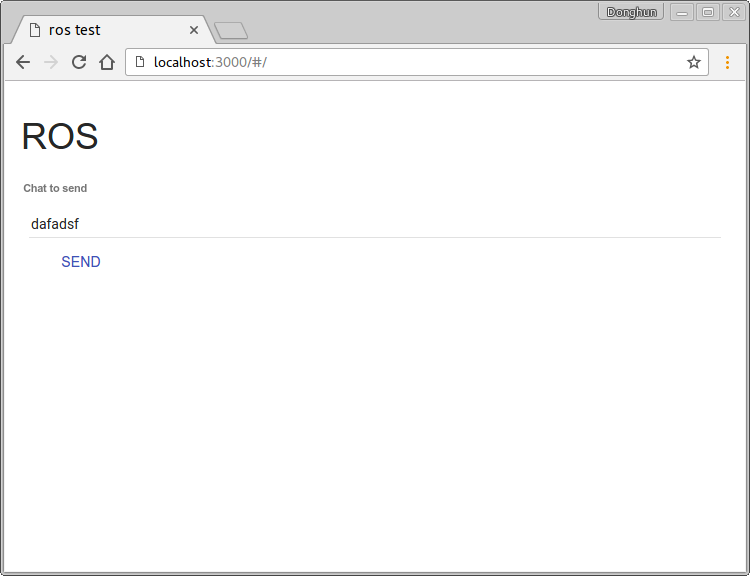
\includegraphics[scale=0.4]{36_webbrowser}
\caption{ROS Websocket Example}
\end{figure}

해당 페이지는 chatter topic으로 위 페이지에 적힌 메세지를 publish하는 웹앱입니다.
echo 명령어를 이용해 chatter 토픽을 보고 있는 상태로 버튼을 눌러보면 실시간으로 데이터가 publish되는 것을 볼 수 있습니다.

그러면 해당 웹앱이 어떻게 구성되어있는지 봅시다. 사실 저 웹앱은 서버가 해주는 일은 웹페이지 로딩밖에 없습니다.
이 작업은 server/index.js 에서 이루어집니다.

\begin{minted}{javascript}
  var express = require('express');
  var router = express.Router();
  var path = require('path');

  router.get('/', function(req, res, next) {
    res.sendFile(path.join(__dirname + '/../views/index.html'));
  });

  module.exports = router;
\end{minted}

그럼 이 javascript 서버 파일이 로딩해주는 index.html 파일을 살펴보면, 여기에서 대부분의 클라이언트 파일의 로딩이 이루어집니다.

\begin{minted}[breaklines=true]{html}
  <!DOCTYPE html>
  <html>
    <head>
      <title>ros test</title>
      <meta name="viewport" content="initial-scale=1"/>
      <link rel='stylesheet' href="https://maxcdn.bootstrapcdn.com/bootstrap/3.3.6/css/bootstrap.min.css" />
      <link rel='stylesheet' href="bower_components/angular-material/angular-material.min.css" />
      <link href='https://fonts.googleapis.com/css?family=Ubuntu' rel='stylesheet' type='text/css'/>
      <link href="https://fonts.googleapis.com/icon?family=Material+Icons" rel="stylesheet"/>

    </head>
    <body >
      <div ng-app="rosTestApp" ui-view >
      </div>
    </body>
    <script src="bower_components/jquery/dist/jquery.min.js" ></script>
    <script src="https://maxcdn.bootstrapcdn.com/bootstrap/3.3.6/js/bootstrap.min.js" ></script>
    <script src="bower_components/angular/angular.min.js" ></script>
    <script src="bower_components/angular-animate/angular-animate.min.js" ></script>
    <script src="bower_components/angular-aria/angular-aria.min.js" ></script>
    <script src="bower_components/angular-messages/angular-messages.min.js" ></script>
    <script src="bower_components/angular-material/angular-material.min.js" ></script>
    <script src="bower_components/angular-ui-router/release/angular-ui-router.min.js" ></script>
    <script src="bower_components/angular-animate/angular-animate.min.js" ></script>
    <script src="bower_components/nipplejs/dist/nipplejs.min.js" ></script>
    <script type="text/javascript" src="http://cdn.robotwebtools.org/EventEmitter2/current/eventemitter2.min.js" ></script>
    <script type="text/javascript" src="http://cdn.robotwebtools.org/roslibjs/current/roslib.min.js" ></script>
    <script type="text/javascript" src="js/ros.js" ></script>
    <script src="app.js" ></script>
    <script src="config.js" ></script>
    <script src="js/controllers/rosTestPage.js" ></script>
    <script src="js/controllers/ros.js" ></script>
    <script src="js/controllers/home.js" ></script>
  </html>

\end{minted}

그리고 앱 페이지 라우팅 설정이 들어가 있는 client/config.js 파일을 열면 처음 라우팅 되는 페이지는 ros라는 이름을 가지고 있고, url은 /인 것을 알 수 있습니다.
그리고 첫 페이지는 rosController라는 함수에 의해 관리되며, 페이지 템플릿은 views/ros.html에 있는 것을 알 수 있죠.

\begin{minted}{javascript}
  rosTestApp.config(function($stateProvider, $urlRouterProvider) {
    //
    // For any unmatched url, redirect to /state1
    $urlRouterProvider.otherwise("/");
    //
    // Now set up the states
    $stateProvider
      .state('home', {
        url: "/home",
        templateUrl: "views/home.html",
        controller : "homeController"
      })
      .state('rosTestPage',{
        url: "/rostest",
        templateUrl: "views/rosTestPage.html",
        controller : "rosTestPageController"
      })
      .state('ros', {
        url: "/",
        templateUrl : "views/ros.html",
        controller : "rosController"
      });
  });
\end{minted}

그러면 이제 ros.html 파일을 열어봅시다. 버튼에 링크되어있는 함수가 sendTopic인 것을 알 수 있습니다. 해당 함수의 패러미터로는 input의 model(charData)이 들어갑니다.

\begin{minted}{html}
  <div class="md-inline-form" layout-padding>
    <h1 >ROS</h1>
    <md-content md-theme="docs-dark" layout-gt-sm="row" layout-padding>
      <md-input-container class="md-block" >
          <label>Chat to send</label>
          <input ng-model="chatData" >
          <md-button class="md-primary" ng-click="sendTopic(chatData)" >SEND</md-button>
      </md-input-container>
    </md-content>
  </div>
\end{minted}

그리고 js/controllers/ros.js 파일을 열면 해당 함수가 실제로 정의되어 있는 것을 알 수 있습니다.

\begin{minted}{javascript}
  rosTestApp.controller("rosController",['$scope',function($scope){
  $scope.sendTopic = function(chatData){
    var chatter = new ROSLIB.Topic(
      {
        ros : ros,
        name : '/chatter',
        messageType : 'std_msgs/String'
      }
    );
    var chat = new ROSLIB.Message(
      {
        data : chatData
      }
    )
    chatter.publish(chat);
  }
}]);$
\end{minted}

위의 함수는 버튼이 눌릴 때 마다 chatter라는 함수를 불러서 /chatter라는 ros topic을 정의하고, data를 input에 있는 데이터로 집어넣은 뒤
publish합니다. 어디로 publish하는지는 처음 웹앱이 실행될 때 로딩되는 스크립트인
js/ros.js 에 있습니다. url/\#/rosTest 에 접속하시면 웹으로 만든 컨트롤러 예제가 나옵니다. 해당 예제를 참고해서 웹앱을 구성해서 컨트롤러를 만들어보시는 것도 좋습니다.

\chapter{ROS Service}

\section{ROS Service 개요}
앞서 이야기했듯이, ROS는 비동기 통신인 Topic 제어 이외에도, 동기 통신 방법을 제공합니다. 그 방법을 ROS에서는 Service라는 이름으로 부르는데, 이러한 Service는 어떻게 구축하는 것인지 알아보도록 합시다.
역시 Service에 대한 보다 자세한 접근은 표윤석 연구원님이 쓰신 책을 참고하시면 좋습니다.

ROS Service는 동기적인 통신방식이기 때문에, request를 보내는 client와 response를 보내는 server로 나뉩니다. ROS의 지금까지 특징으로 미루어보면 쉽게 짐작하실 수 있겠지만,
둘은 사용 언어나 플랫폼이 전혀 달라도 됩니다. bash에서 python 프로그램의 service를 call할 수도 있고, 반대의 경우도 가능합니다.


\begin{figure}[h]
\centering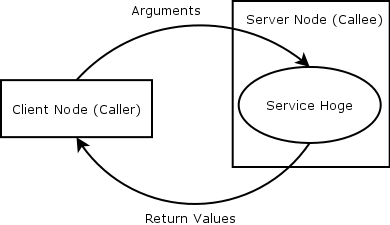
\includegraphics[scale=0.7]{37_service}
\caption{ros service 구성}
\end{figure}

Service를 제공하는 서버 노드에 Argument와 함께 요청이 들어오면, 연산 후 Return 값을 서버는 클라이언트 노드에 보냅니다.
이것이 기본적인 서비스의 작동 방식입니다.

\section{ROS Service 실습}

서비스의 개념을 잡기 위해 간단한 실습을 해봅시다. 먼저 gazebo를 켭니다.

\begin{minted}{bash}
  rosrun gazebo_ros gazebo
\end{minted}

그리고 아래 커멘드를 통해 현재 service가 어떤 것들이 있는지 파악합니다.

\begin{minted}{bash}
  rosservice list
\end{minted}

그러면 gazebo에 연결된 여러 서비스들이 나올 것입니다. gazebo에 아래와 같이 box를 하나 놓은 후
이 box에 service를 이용해 torque를 가해 봅시다.

\begin{figure}[h]
\centering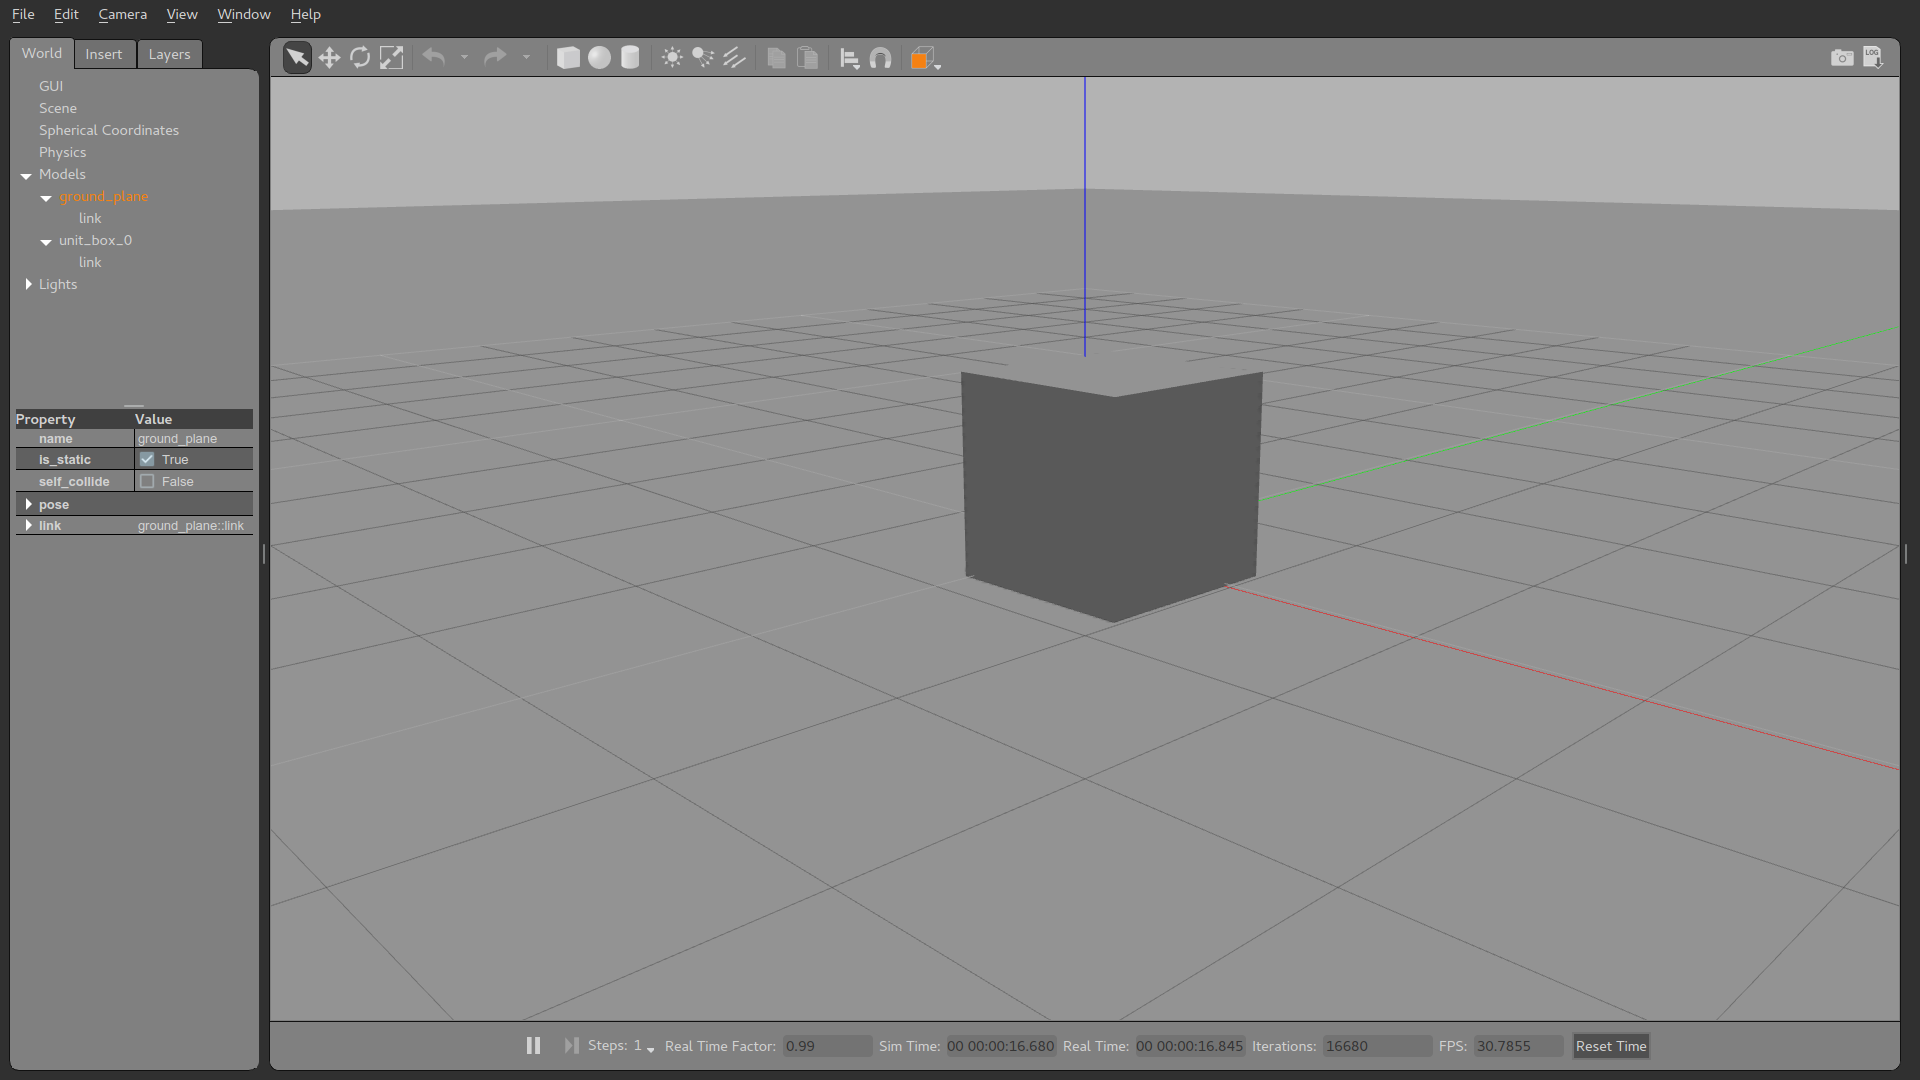
\includegraphics[scale=0.23]{38_gazebo_box}
\caption{gazebo}
\end{figure}

\begin{minted}{bash}
  rosservice call /gazebo/apply_body_wrench "body_name: 'unit_box_0::link'
    reference_frame: ''
    reference_point: {x: 0.0, y: 0.0, z: 0.0}
    wrench:
      force: {x: 0.0, y: 0.0, z: 0.0}
      torque: {x: 0.0, y: 0.0, z: 7.0}
    start_time: {secs: 0, nsecs: 0}
    duration: {secs: 5, nsecs: 0}"
\end{minted}

bash를 통해 위와 같이 서비스를 호출하면 서비스 호출이 되었을 경우 Success : True 로 나옵니다.
그리고 box 모델이 회전을 시작하죠.
해당 서비스는 호출했을 시에 gazebo 안의 모델의 물리적 간섭을 서비스 호출 시 넘겨준 패러미터대로 하고,
서비스 리턴 값으로는 성공/ 실패 여부를 내보냅니다. 따라서 서비스는 어떤 데이터가 확실히 넘어갔는지 알 수 있는 점에서 topic 기반 통신과 차이점을 가지죠.

% This is an example of theorems.
%
% \subsection{Several equations}\index{Theorems!Several Equations}
% This is a theorem consisting of several equations.
%
% \begin{theorem}[Name of the theorem]
% In $E=\mathbb{R}^n$ all norms are equivalent. It has the properties:
% \begin{align}
% & \big| ||\mahbf{x}|| - ||\mathbf{y}|| \big|\leq || \mathbf{x}- \mathbf{y}||\\
% &  ||\sum_{i=1}^n\mathbf{x}_i||\leq \sum_{i=1}^n||\mathbf{x}_i||\quad\text{where $n$ is a finite integer}
% \end{align}
% \end{theorem}
%
% \subsection{Single Line}\index{Theorems!Single Line}
% This is a theorem consisting of just one line.
%
% \begin{theorem}
% A set $\mathcal{D}(G)$ in dense in $L^2(G)$, $|\cdot|_0$.
% \end{theorem}

%------------------------------------------------
%
% \section{Definitions}\index{Definitions}
%
% This is an example of a definition. A definition could be mathematical or it could define a concept.
%
% \begin{definition}[Definition name]
% Given a vector space $E$, a norm on $E$ is an application, denoted $||\cdot||$, $E$ in $\mathbb{R}^+=[0,+\infty[$ such that:
% \begin{align}
% & ||\mathbf{x}||=0\ \Rightarrow\ \mathbf{x}=\mathbf{0}\\
% & ||\lambda \mathbf{x}||=|\lambda|\cdot ||\mathbf{x}||\\
% & ||\mathbf{x}+\mathbf{y}||\leq ||\mathbf{x}||+||\mathbf{y}||
% \end{align}
% \end{definition}
%
% %------------------------------------------------
%
% \section{Notations}\index{Notations}
%
% \begin{notation}
% Given an open subset $G$ of $\mathbb{R}^n$, the set of functions $\varphi$ are:
% \begin{enumerate}
% \item Bounded support $G$;
% \item Infinitely differentiable;
% \end{enumerate}
% a vector space is denoted by $\mathcal{D}(G)$.
% \end{notation}
%
% %------------------------------------------------
%
% \section{Remarks}\index{Remarks}
%
% This is an example of a remark.
%
% \begin{remark}
% The concepts presented here are now in conventional employment in mathematics. Vector spaces are taken over the field $\mathbb{K}=\mathbb{R}$, however, established properties are easily extended to $\mathbb{K}=\mathbb{C}$.
% \end{remark}
%
% %------------------------------------------------
%
% \section{Corollaries}\index{Corollaries}
%
% This is an example of a corollary.
%
% \begin{corollary}[Corollary name]
% The concepts presented here are now in conventional employment in mathematics. Vector spaces are taken over the field $\mathbb{K}=\mathbb{R}$, however, established properties are easily extended to $\mathbb{K}=\mathbb{C}$.
% \end{corollary}
%
% %------------------------------------------------
%
% \section{Propositions}\index{Propositions}
%
% This is an example of propositions.
%
% \subsection{Several equations}\index{Propositions!Several Equations}
%
% \begin{proposition}[Proposition name]
% It has the properties:
% \begin{align}
% & \big| ||\mathbf{x}|| - ||\mathbf{y}|| \big|\leq || \mathbf{x}- \mathbf{y}||\\
% &  ||\sum_{i=1}^n\mathbf{x}_i||\leq \sum_{i=1}^n||\mathbf{x}_i||\quad\text{where $n$ is a finite integer}
% \end{align}
% \end{proposition}
%
% \subsection{Single Line}\index{Propositions!Single Line}
%
% \begin{proposition}
% Let $f,g\in L^2(G)$; if $\forall \varphi\in\mathcal{D}(G)$, $(f,\varphi)_0=(g,\varphi)_0$ then $f = g$.
% \end{proposition}
%
% %------------------------------------------------
%
% \section{Examples}\index{Examples}
%
% This is an example of examples.
%
% \subsection{Equation and Text}\index{Examples!Equation and Text}
%
% \begin{example}
% Let $G=\{x\in\mathbb{R}^2:|x|<3\}$ and denoted by: $x^0=(1,1)$; consider the function:
% \begin{equation}
% f(x)=\left\{\begin{aligned} & \mathrm{e}^{|x|} & & \text{si $|x-x^0|\leq 1/2$}\\
% & 0 & & \text{si $|x-x^0|> 1/2$}\end{aligned}\right.
% \end{equation}
% The function $f$ has bounded support, we can take $A=\{x\in\mathbb{R}^2:|x-x^0|\leq 1/2+\epsilon\}$ for all $\epsilon\in\intoo{0}{5/2-\sqrt{2}}$.
% \end{example}
%
% \subsection{Paragraph of Text}\index{Examples!Paragraph of Text}
%
% \begin{example}[Example name]
% \lipsum[2]
% \end{example}
%
% %------------------------------------------------
%
% \section{Exercises}\index{Exercises}
%
% This is an example of an exercise.
%
% \begin{exercise}
% This is a good place to ask a question to test learning progress or further cement ideas into students' minds.
% \end{exercise}
%
% %------------------------------------------------
%
% \section{Problems}\index{Problems}
%
% \begin{problem}
% What is the average airspeed velocity of an unladen swallow?
% \end{problem}
%
% %------------------------------------------------
%
% \section{Vocabulary}\index{Vocabulary}
%
% Define a word to improve a students' vocabulary.
%
% \begin{vocabulary}[Word]
% Definition of word.
% \end{vocabulary}
%
% %----------------------------------------------------------------------------------------
% %	PART
% %----------------------------------------------------------------------------------------
%
% \part{Part Two}
%
% %----------------------------------------------------------------------------------------
% %	CHAPTER 3
% %----------------------------------------------------------------------------------------
%
% \chapterimage{chapter_head_1.pdf} % Chapter heading image
%
% \chapter{Presenting Information}
%
% \section{Table}\index{Table}
%
% \begin{table}[h]
% \centering
% \begin{tabular}{l l l}
% \toprule
% \textbf{Treatments} & \textbf{Response 1} & \textbf{Response 2}\\
% \midrule
% Treatment 1 & 0.0003262 & 0.562 \\
% Treatment 2 & 0.0015681 & 0.910 \\
% Treatment 3 & 0.0009271 & 0.296 \\
% \bottomrule
% \end{tabular}
% \caption{Table caption}
% \end{table}
%
% %------------------------------------------------
%
% \section{Figure}\index{Figure}
%
% \begin{figure}[h]
% \centering
\includegraphics[scale=0.5]{placeholder}
% \caption{Figure caption}
% \end{figure}

%----------------------------------------------------------------------------------------
%	BIBLIOGRAPHY
%----------------------------------------------------------------------------------------

\chapter*{Bibliography}
\addcontentsline{toc}{chapter}{\textcolor{ocre}{Bibliography}}
\section*{Books}
\addcontentsline{toc}{section}{Books}
\printbibliography[heading=bibempty,type=book]
\section*{Articles}
\addcontentsline{toc}{section}{Articles}
\printbibliography[heading=bibempty,type=article]

%----------------------------------------------------------------------------------------
%	INDEX
%----------------------------------------------------------------------------------------

\cleardoublepage
\phantomsection
\setlength{\columnsep}{0.75cm}
\addcontentsline{toc}{chapter}{\textcolor{ocre}{Index}}
\printindex

%----------------------------------------------------------------------------------------

\end{document}
